%------------------------------------------------------------------
\section{Introduction générale}

Dans les modèles quantiques intégrables, l’évolution vers l’équilibre, à partir d’un état initial arbitraire (et typiquement hors d’équilibre), ne conduit pas à une thermique de Gibbs classique.  
En effet, du fait de l’existence d’une infinité de charges conservées en involution, les systèmes intégrables n’explorent qu’une sous-partie contrainte de l’espace des états accessibles.  
Ils relaxent alors vers un état stationnaire décrit par une \emph{Ensemble Thermodynamique Généralisé} (GGE), qui encode la conservation de toutes ces quantités.

Cette section pose les fondations nécessaires à la description de ces états stationnaires dans le cadre de la \textbf{thermodynamique de Bethe} (TBA), qui généralise l’analyse au-delà de l’état fondamental.  
Nous considérons ici un régime macroscopique à température (ou entropie) finie, correspondant à des états hautement excités du spectre, mais toujours décrits dans le formalisme intégrable exact.

Notre point de départ est la relation constitutive entre la densité de \emph{quasi-particules} (ou rapidités) $\rho(\theta)$ et la densité d’états disponibles $\rho_s(\theta)$, qui encode le spectre accessible en présence d’interactions.  
Nous introduisons ensuite une opération clé de la TBA, appelée \emph{habillage} (\emph{dressing}), qui intervient systématiquement dans le calcul des observables physiques et permet de prendre en compte de manière non perturbative les effets des interactions.  
Cette construction sera illustrée dans le cadre du modèle intégrable de Lieb–Liniger, qui décrit un gaz unidimensionnel de bosons avec interaction delta répulsive.

Les outils développés ici seront fondamentaux pour formuler dans la section suivante le concept d’ensemble généralisé (GGE), et pour décrire la dynamique de relaxation des systèmes intégrables.


%------------------------------------------------------------------
\subsection{Limite thermodynamique}

Dans la limite thermodynamique $N,L\to\infty$ à densité finie
$N/L=\text{cst}$, les équations de Bethe discrètes se condensent en une
équation intégrale pour les densités de rapidités :
\begin{equation}
2\pi \rho_s \;=\; 1 \;+\;\Delta \star \rho,
\label{eq:TBA-rhos}
\end{equation}
où le symbole 
\(
[\Delta \star \rho](\theta)
\)
désigne la \textbf{convolution}
\[
[\Delta \star \rho](\theta)\;=\; \int_{-\infty}^{\infty}
      \!d\theta'\; \Delta(\theta-\theta')\,\rho(\theta').
\]
Pour le modèle de \textbf{Lieb–Liniger} de couplage $g>0$.  
%le noyau
%\(
%\Delta(\theta)=\dfrac{2g}{\theta^{2}+g^{2}}
%\)
%provient de la dérivée de la phase de diffusion
%$S(\theta)=\dfrac{\theta-ic}{\theta+ic}$.

%------------------------------------------------------------------
\subsection{Opération de \emph{dressing}}
\label{sec:dressing}

\subsubsection{Définition}

À toute fonction  $f(\theta)$ on associe sa version \emph{habillée}
$f^{\mathrm{dr}}(\theta)$, solution de l’équation intégrale
%\begin{align}
%f^{\mathrm{dr}}(\theta) &= f(\theta) \;+\;
%       \int_{-\infty}^{\infty}\!\frac{d\theta'}{2\pi}\;
%             \Delta(\theta-\theta')\,\nu(\theta')\,f^{\mathrm{dr}}(\theta')
%\nonumber\\
%&= f(\theta)\;+\;\Bigl[\tfrac{\Delta}{2\pi}\star\bigl(\nu\,f^{\mathrm{dr}}\bigr)
%     \Bigr](\theta),
%\label{eq:dressing}
%\end{align}
\begin{eqnarray}
	f^{\mathrm{dr}} & = & f  \;+\;\Bigl[\tfrac{\Delta}{2\pi}\star\bigl(\nu\,f^{\mathrm{dr}}\bigr)\Bigr] \label{eq:dressing}	
\end{eqnarray}
où $\Delta/2\pi$ est un noyau de convolution spécifique et 
\(
\nu=\dfrac{\rho}{\rho_s}
\)
est le \emph{facteur d’occupation}.

\subsubsection{Interprétation physique}

Le dressing incorpore \emph{à tous ordres} les rétrodiffusions entre
quasi‑particules ; il encode ainsi les corrections
d’interaction aux grandeurs physiques initiales $f(\theta)$.
Dans le Lieb–Liniger, on l’utilise pour obtenir :

* l’énergie habillée $\varepsilon^{\mathrm{dr}}(\theta)$,
* la charge impulsion $p^{\mathrm{dr}}(\theta)$,
* les susceptibilités (voir chap.\,\ref{chap:GGE}).

\subsubsection{Exemple\,: densité de sites}

En posant $f(\theta)=1$, l’équation~\eqref{eq:dressing} donne
\(
1^{\mathrm{dr}}=1+\frac{\Delta}{2\pi}\star\bigl(\nu\,1^{\mathrm{dr}}\bigr)
\) soit 
\[
2\pi\rho_s=1^{\mathrm{dr}},
\]
ce qui n’est autre que la
relation constitutive~\eqref{eq:TBA-rhos}.

\vspace{1ex}
La formalisation ci‑dessus fournit la brique de base pour la
\textbf{hydrodynamique généralisée} et, dans la section suivante, pour la
définition précise de l’\textbf{Ensemble d’Équilibre Généralised (GGE)}
assurant la relaxation des systèmes intégrables hors‑équilibre.

%%Dans ce chapitre, nous nous intéressons aux fluctuations de la distribution de rapidité \( \delta \rho \) autour d'une distribution de référence \( \rho^c \), qui maximise la contribution à la fonction de partition des états, exprimée comme une fonctionnelle de la distribution \( \rho \) : 

La fonction de partition des états, s'exprime comme une fonctionnelle de la distribution \( \rho \) : 

\begin{eqnarray*}
	\Xi & = & \sum_\rho \exp \left( -\mathcal{A}(\rho) \right).
\end{eqnarray*}  

Dans la section {\em \bf Entropie de Yang-Yang} (\ref{??}), l'action \( \mathcal{A}(\rho) \) s'écrit sous la forme :  

\begin{eqnarray*}
	\mathcal{A}(\rho) & \doteq & - L\mathcal{S}_{YY}(\rho) + L\int f(\theta) \rho (\theta) \, d\theta,		
\end{eqnarray*}  

où \( \mathcal{S}_{YY} \) est la fonctionnelle d'entropie de Yang-Yang, définie dans (\ref{??}), et \( f \) est la fonction paramétrant les charges, introduite dans (\ref{??}).  

Dans cette même section {\em \bf Entropie de Yang-Yang} (\ref{??}), nous avons établi un lien entre \( f \) et distribution de référence \( \rho^c \), qui maximise la contribution à la fonction de partition des états .\\

On veux tester si nos experience est décrit pas un GGE. Pour cela nous nous intéressons aux fluctuations de la distribution de rapidité \( \delta \rho \) autour \( \rho^c \).

%Nous poursuivons à présent avec cette définition de l'action de classe $\mathcal{C}^2$ et admetant une distribution critique $\rho^c$ tel que sa différentielle en ce point critique soit nulle $d\mathcal{A}_{\rho^c} = 0 $ (\ref{??}) de sorte que d'aprés la formule de Taylor-Youg %afin de déterminer les fluctuations autour de \( \Pi^c \). Pour cela, nous réécrivons l'action sous la forme :  

Nous poursuivons à présent avec cette définition de l'action de classe $\mathcal{C}^2$ et admetant une distribution critique $\rho^c$ tel que sa différentielle en ce point critique soit nulle $d\mathcal{A}_{\rho^c} = 0 $ (\ref{??}) de sorte que d'aprés la formule de Taylor-Youg %afin de déterminer les fluctuations autour de \( \Pi^c \). Pour cela, nous réécrivons l'action sous la forme :  

\begin{eqnarray*}  
	\mathcal{A}(\rho^c + \delta \rho) & \underset{ \delta \rho \to 0 }{=} & \mathcal{A}(\rho^c)  + \frac{1}{2} \left. \frac{\delta^2 \mathcal{A}}{\delta \rho^2} \right|_{\rho^c} (\delta \rho) + \mathcal{O}((\delta \rho)^3),  
\end{eqnarray*}  

une expression quadratique pour l'action à l'ordre dominant en \( \delta \Pi \) avec $\left. \frac{\delta^2 \mathcal{A}}{\delta \rho^2} \right|_{\rho^c}$ la forme quadratique définie positive (Fig (\ref{fig.fluctu.A})).

\begin{figure}[H]
	\centering 
	\begin{tikzpicture}
		\begin{scope}[shift={(0,0)}]
			\begin{scope}[transform canvas={scale=0.6}]
				% Définition des couleurs avec les codes HTML
\definecolor{colorOne}{HTML}{443E46}
\definecolor{colorTwo}{HTML}{F6DEB8}
\definecolor{colorThree}{HTML}{908CA4}
\definecolor{colorFour}{HTML}{57659E}
\definecolor{colorFive}{HTML}{C57284}
\definecolor{colorSix}{HTML}{FF5B69}

% Raccourcis pour les couleurs
\def\colorOne{colorOne}
\def\colorTwo{colorTwo}
\def\colorThree{colorThree}
\def\colorFour{colorFour}
\def\colorFive{colorFive}
\def\colorSix{colorSix}

\def\colorslide{blue!50!black}



\begin{scope}
	% Tracer une courbe lisse entre des points
	\draw[shift={(0,0)} ,\colorOne]
		(-1 , 0 ) edge [thick,line width=0.8ex , ->,>=triangle 45  , \colorOne] node [pos = 1 , below ]{\huge$\rho$}( 5  , 0 )
	;
	\draw[shift={(0,0)}, color=\colorOne]
		(0, -1.0 ) edge [thick,line width=0.8ex , ->,>=triangle 45  ]node [pos=0.9,left=0.2cm ]{\huge$\mathcal{A}(\rho)$}( 0  , 5 )
	;
	\draw[]
		(2.5, 0.12 ) edge [thick,line width=0.8ex ,\colorThree ]node [pos=1,below  ]{\huge$\rho^c$} (2.5, -0.12 )	
	;
	
	\draw[]
		(2.5, -0.12 ) edge [thick,line width=0.4ex , dashed, \colorThree ] (2.5, 5.5 )
		(1.5, 1 ) edge [thick,line width=0.4ex , <->,>=triangle 45  , \colorThree ] (3.5, 1 )
		(-0.3,1) edge [thick,line width=0.4ex  , \colorThree ] node [pos=0,left ]{\huge$\mathcal{A}(\rho^c)$} (0.3, 1 )	
	;
    \draw[thick, line width=0.8ex , \colorFour] plot[smooth, tension=0.7] coordinates {
        (1, 5) (1.6 , 3 ) (2.5, 1) (3.5 , 3 )  (4, 5)
    };		
	
\end{scope}

	
			
			\end{scope}
			
			\draw[color = red , scale = 0.5 , draw = none  ] (-2 , -1) rectangle (5, 6) ; 	
		\end{scope}
		
		\begin{scope}[shift={(19,-1)}]
			\begin{scope}[transform canvas={scale=0.6}]
				% Définition des couleurs avec les codes HTML
\definecolor{colorOne}{HTML}{443E46}
\definecolor{colorTwo}{HTML}{F6DEB8}
\definecolor{colorThree}{HTML}{908CA4}
\definecolor{colorFour}{HTML}{57659E}
\definecolor{colorFive}{HTML}{C57284}
\definecolor{colorSix}{HTML}{FF5B69}

% Raccourcis pour les couleurs
\def\colorOne{colorOne}
\def\colorTwo{colorTwo}
\def\colorThree{colorThree}
\def\colorFour{colorFour}
\def\colorFive{colorFive}
\def\colorSix{colorSix}

\def\colorslide{blue!50!black}

\def\Occupation{
	\def\traitx{0.3}
	\def\traity{0.5}
	\draw[shift={(0,0)}]
		(-13.5 , 0 ) edge [thick,line width=0.8ex ]( -3.2  , 0 )
		( -3.2 - \traitx  , 0 - \traity ) edge [thick,line width=0.8ex ]( -3.2 + \traitx  , 0 + \traity  )
		( -2.8 - \traitx  , 0 - \traity ) edge [thick,line width=0.8ex ]( -2.8 + \traitx  , 0 + \traity  )
		(-2.8 , 0 ) edge [thick,line width=0.8ex ](2.8  , 0 )
		( 2.8 - \traitx  , 0 - \traity ) edge [thick,line width=0.8ex ]( 2.8 + \traitx  , 0 + \traity  )
		( 3.2 - \traitx  , 0 - \traity ) edge [thick,line width=0.8ex ]( 3.2 + \traitx  , 0 + \traity  )
		(3.2, 0 ) edge [thick,line width=0.8ex,->,>=triangle 45 , color = black ]node [pos=1.01,below  ]{\huge$\theta$}	( 13  , 0 )
	;
	\draw[shift={(0,0)}, color=\colorOne]
		(-10.5 , -1.5 ) edge [thick,line width=0.8ex , ->,>=triangle 45  ]( -10.5  , 4.5 )
	;
		
	\foreach \r in {1 , ... , 3 } {
%		\draw[
%		decoration={
%		markings,
%    	mark connection node=my node,
%    	mark=at position 0 with{\node [blue,transform shape] (my node) {\large \r};}},
%		color=gray, thick, 
%		line width=0.5ex] decorate { 
%            (-11.0, \r) -- (-10.1, \r )}
%        ;
        \draw[
			color=\colorOne,
			] 
            (-11.0, \r) edge[color=\colorThree , thick,line width=0.5ex] node [pos=-0.5 ]{\large\color{\colorFour} $\frac{\r}{\delta \theta}$ } (-10.3, \r )
        	;
	
	}
	

	
	% Graduation abcsisse 
	% Définitions des listes
% Definitions of the lists
\def\listetuple{-9/\theta_{1}, -8/\theta_{2} , -5/\theta_{3} , -2/\theta_{a-1} , 0/\theta_{a} , 1/\theta_{a+1} , 2/\theta_{a+2} ,  5/\theta_{N-4} , 7/\theta_{N-3},8/\theta_{N-1},9/\theta_{N} }
\def\listetrais{-12 , -11, -10, -9 , -8 , -7 ,  -6 , -5, -4.5,-4, -2 , -1, 0 , 0.5, 1, 2, 4 , 5 ,  6 , 7 , 8 ,8.5, 9 ,  10 , 11, 12 }

% Loop over listetrais
\foreach \r in \listetrais {
    % Initialize found variable to zero
    % Initialize found variable to zero
    %\pgfmathsetmacro\found{0}
    \global\def\found{0}
    \xdef\nomtheta{}
    
    % Check if \r is in listetuple
    \foreach \x/\y in \listetuple { 
        \ifdim \r pt=\x pt % If \r matches any \x in listetuple
            \global\def\found{1} ;
            \xdef\nomtheta{\y} % Set \nomtheta to the corresponding \y
            %\pgfmathsetmacro\found{1} % Set found to 1            
            %\global\pgfmathsetmacro\found{1}
        \fi
    }
    
    %\node [circle, draw, red] (A) at (\r, 2) {\found , $\nomtheta$};
    
    % Draw the line and display \nomtheta if found
    \ifnum\found=1
        \draw[color=\colorOne, thick, line width=0.5ex] 
            (\r, -0.3) -- (\r, 0.3) node[red , pos=-0.5] {\large $\nomtheta$};
         \filldraw[line width=0.5ex, color=\colorSix, outer color=\colorSix, inner color=\colorSix] 
            (\r, 0) circle (4pt);
    \else 
        % Draw without \nomtheta and add a blue circle if not found
        \draw[color=\colorOne, thick, line width=0.5ex] 
            (\r, -0.3) -- (\r, 0.3);
        \filldraw[line width=0.5ex, color=\colorSix, outer color=\colorTwo, inner color=\colorTwo] 
            (\r, 0) circle (4pt); 
    \fi
}

\def\listetrais{-9.5/\theta_{i-1}/2/3, -6.5/\theta_{i}/1/4  ,   -1.5/\theta_{j}/2/4 , 1.5/\theta_{j+1}/-1/3 , 3.5/\theta_{\ell-1}/1/3 , 6.5/\theta_{\ell}/3/4 , 9.5/\theta(\theta_{\ell+1})/-1/3 };



\foreach \r/\nomx/\y/\ys in \listetrais {
	\draw[
		decoration={
		markings,
    	mark connection node=my node,
    	mark=at position .5 with{\node [blue,transform shape] (my node) {\large \color{\colorFour} $\nomx$};}},
		color=\colorThree , thick, 
		line width=0.5ex] decorate { 
            (\r, 0.12) -- (\r, -1.2)}
        ;
     
     \ifdim \y pt > -1 pt 
     	\draw[
			decoration={
			markings,
    		mark connection node=my node,
    		mark=at position .5 with{\node [blue,transform shape] (my node) {\large \color{\colorFour} $\Pi(\nomx) $};}},
			color=\colorThree, thick, 
			line width=0.5ex] decorate { 
            (\r, \y) -- (\r +3, \y)}
        ;
        \draw[
			decoration={
			markings,
    		mark connection node=my node,
    		mark=at position .5 with{\node [blue,transform shape] (my node) {\large \color{\colorFive} $\Pi_s(\nomx) $};}},
			color=\colorFive, thick, 
			line width=0.5ex] decorate { 
            (\r, \ys) -- (\r +3, \ys)}
        ;
     \fi 
     \ifdim \r pt= -1.5 pt
     	\draw[
     		decoration={
			markings,
    		mark connection node=my node,
    		mark=at position .5 with{\node [blue,transform shape] (my node) {\large \color{\colorFour}  $\delta \theta $};},
    		%mark=at position 0.1  with {\arrow[blue, line width=0.5ex]{<}},
    		%mark=at position 1  with {\arrow[blue, line width=0.5ex]{>}}
    		},
        	color=\colorThree,
        	thick,
        	line width=0.5ex,
        	%arrows={Computer Modern Rightarrow[line cap=round]-Computer Modern Rightarrow[line cap=round]}
   			](\r, -1.2) edge[arrows={Computer Modern Rightarrow[line cap=round]-}] (\r + 0.4, -1.2)decorate {
    		(\r, -1.2) -- (\r + 3, -1.2)}(\r + 2, -1.2) edge[arrows={-Computer Modern Rightarrow[line cap=round]}] (\r + 3, -1.2)
    		;
    \fi
			
	
}


			
}


\begin{scope}
	%\draw[help lines , width=1.5ex] (-8,-3) grid (8,3);\draw[help lines ,width=0.5ex , opacity = 0.5] (-3,-3) grid[step=0.1] (3,3));
	
	%\draw[help lines] 
	%	(-3,-3) edge[width=1.5ex] grid (3,3)	
	%	(-3,-3) edge[width=0.5ex , opacity = 0.5] grid (3,3)	
	%;
	\begin{scope}[shift={(0,1)},rotate=0,opacity=1,color=black]
		\Occupation	
		
		%\node[anchor=east, font=\bfseries] at (-11, 0) {\color{red}\large (T = 0 )} ;	
	\end{scope}
	
	
	
	
	\begin{scope}[shift={(-10.5,7)},rotate=0,opacity=1,color=black]
	
	\begin{scope}[shift={(-0,0)},rotate=0,opacity=1,color=black]
	
		\draw[shift={(0,0)} ,line width=1ex,rounded corners = 1ex,color=\colorOne , opacity =1 ,fill=\colorOne!00 , pattern={north east lines} , pattern color=\colorOne!00 ]
			(0 , -1 ) rectangle (5,1)
		;
		

		\begin{scope}[shift={(0.5,0.5)}]
			\draw[color=\colorOne, thick, line width=0.5ex] 
            (0, -0.3) -- (0, 0.3) ;
            \filldraw[line width=0.5ex, color=\colorSix, outer color=\colorSix, inner color=\colorSix] 
            (0, 0) circle (4pt);
            
            \node[anchor=west, font=\bfseries] at (0.2, 0) {\color{\colorSix}\large : quasi-particule};
		\end{scope}
		
		\begin{scope}[shift={(0.5,-0.5)}]
			\draw[color=\colorOne, thick, line width=0.5ex] 
            (0, -0.3) -- (0, 0.3) ;
            \filldraw[line width=0.5ex, color=\colorSix, outer color=\colorTwo, inner color=\colorTwo] 
            (0, 0) circle (4pt);
            
            \node[anchor=west, font=\bfseries] at (0.2, 0) {\color{\colorSix}\large : hole};
		\end{scope}

	\end{scope}
	
	\begin{scope}[shift={(6,0)},rotate=0,opacity=1,color=black]	
		
		\draw[shift={(0,0)} ,line width=1ex,rounded corners = 1ex,color=\colorOne , opacity =1 ,fill=\colorOne!00 , pattern={north east lines} , pattern color=\colorOne!00 ]
			(0 , -1 ) rectangle (7.5,1)
		;
		
		\node[anchor=west] at (0.5, 0.5) {\color{\colorFour}\large $\Pi$ };\node[anchor=west, font=\bfseries] at (1, 0.5) {\color{\colorFour}\large : quasi-particule distribution};
		
		\node[anchor=west] at (0.5, -0.5) {\color{\colorFour}\large $\Pi_h$ };\node[anchor=west, font=\bfseries] at (1, -0.5) {\color{\colorFour}\large  : hole distribution};
		
	\end{scope}
	
	\begin{scope}[shift={(14.5,0)},rotate=0,opacity=1,color=black]	
		
		\draw[shift={(0,0)} ,line width=1ex,rounded corners = 1ex,color=\colorOne , opacity =1 ,fill=\colorOne!00 , pattern={north east lines} , pattern color=\colorOne!00 ]
			(0 , -0.5 ) rectangle (7.0,0.5)
		;
		
		\node[anchor=west] at (0.2, 0) {\color{\colorFour}\large ${\color{\colorFive}\Pi_s} = \Pi + \Pi_h $ } node[anchor=west , font=\bfseries] at (3.1 , 0 )  {\color{\colorFour}\large {\color{\colorFive} : density of states}};
		
	\end{scope}
	
	
	\end{scope}


		
	
\end{scope}

	
			
			\end{scope}
			\begin{scope}[scale=1]
				\draw[color = red , scale = 1 , draw = none  ] (-1 , -1) rectangle (5, 5) ; 
			\end{scope}	
		\end{scope}

		
				
			
	\end{tikzpicture}	
	\captionsetup{skip=10pt} % Ajoute de l’espace après la légende
	\label{fig.fluctu.A}
\end{figure}


On discrétise l'axe des rapidités en  petite cellule de rapidité $[\theta, \theta+\delta\theta]$, qui contient $L\rho(\theta) \delta \theta$ rapidités. 
	



Avec ces petites tranches, la forme quadratique s’écrit :

\begin{eqnarray*}
    \left. \frac{\delta^2 \mathcal{A}}{{\delta \rho}^2} \right|_{\rho^c}(\delta \rho ) &=&  \sum_{a,b \mid \text{tranche}}  
    \delta \rho(\theta_a)  \frac{\partial^2 \mathcal{A}}{\partial \delta \rho(\theta_a) \partial \delta \rho(\theta_b) } (\rho^c)  \delta \rho(\theta_b).
\end{eqnarray*}
Les fluctuations s’écrivent donc :

\begin{eqnarray*}
    \langle \delta \rho ( \theta) \delta \rho ( \theta') \rangle &=&  
    \frac{ \int d\delta \rho \, \delta \rho(\theta) \delta \rho ( \theta') 
    \exp \left( - \frac{1}{2} \sum_{a,b \mid \text{tranche}}  
    \delta \rho(\theta_a) \frac{\partial^2 \mathcal{A}}{\partial \delta \rho(\theta_a) \partial \delta \rho(\theta_b) } (\rho^c)  \delta \rho(\theta_b) \right) }
    { \int d\delta \Pi  
    \exp \left( - \frac{1}{2} \sum_{a,b \mid \text{tranche}}  
    \delta \rho(\theta_a) \frac{\partial^2 \mathcal{A}}{\partial \delta \rho(\theta_a) \partial \delta \rho(\theta_b) } (\rho^c)  \delta \rho(\theta_b) \right) } \\
    &=& \left( \mathbf{A}^{-1} \right)_{\theta , \theta'}
\end{eqnarray*}


\begin{aff}

\begin{eqnarray*}
	\langle \delta \rho ( \theta) \delta \rho ( \theta') \rangle &=& 	\left( \mathbf{A}^{-1} \right)_{\theta , \theta'}
\end{eqnarray*}

	
avec la  {\em matrice hessienne} $\mathbf{A}_{\theta , \theta'} \equiv \frac{\partial^2 \mathcal{A}}{\partial \delta \rho(\theta) \partial \delta \rho(\theta') }(\rho^c)$, au point critique/ qui maximise la probabilité  $\rho^c=\rho^c_s \nu^c $, s'écrit

\begin{eqnarray*}
	\operator{A} & = & \operator{A}^{(0)} + \delta \theta \operator{V}
\end{eqnarray*}

avec 

\begin{eqnarray*}
	A^{(0)}_{\theta , \theta'}  & = &  L\delta \theta \left ( \frac{ 1}{\rho^c_s ( 1  - \nu^c ) \nu^c } \right )(\theta)    \delta({\theta - \theta '})	,\\
	V_{\theta , \theta'}  &= & L \delta \theta \left \{ - \left [ \left ( \frac{1}{\rho^c_s( 1 - \nu^c) } \right ) ( \theta)  +  \left ( \frac{1}{\rho^c_s( 1 - \nu^c) } \right ) ( \theta' )\right ] \frac{ \Delta( \theta'- \theta )}{ 2 \pi } + \int d\theta''  \left ( \frac{\nu^c}{\rho^c_s( 1 - \nu^c) } \right )(\theta'') \frac{\Delta(\theta''- \theta)}{2 \pi}\frac{\Delta(\theta''- \theta')}{2 \pi}   \right \} 	
\end{eqnarray*}

\end{aff}

\subsection{Testes}

\begin{eqnarray*}
	\Delta_{\operator{\mathcal{N}}}^2  & = &  \frac{1}{\beta} \left . \frac{\partial \langle \operator{\mathcal{N}} \rangle}{\partial \mu} \right )_T \\
	\Delta_{\operator{\mathcal{E}}-\mu \operator{\mathcal{N}}}^2  & = &  - \left . \frac{\partial \langle \operator{\mathcal{E}}-\mu \operator{\mathcal{N}} \rangle}{\partial \beta} \right )_\mu 
\end{eqnarray*}

et 

\begin{eqnarray*}
	\Delta_{\operator{\mathcal{N}}}^2  &= & L^2 \int d\theta_a \int d \theta_b \, \langle \delta \rho(\theta_a) \delta \rho(\theta_b) \rangle \\
	\Delta_{\operator{\mathcal{E}}-\mu \operator{\mathcal{N}}}^2  & = & L^2 \int d\theta_a \int d \theta_b \, \left ( - \mu + \frac{1}2 m \theta_a^2  \right  )\left ( - \mu + \frac{1}2 m \theta_b^2  \right  )  \langle \delta \rho(\theta_a) \delta \rho(\theta_b) \rangle
\end{eqnarray*}

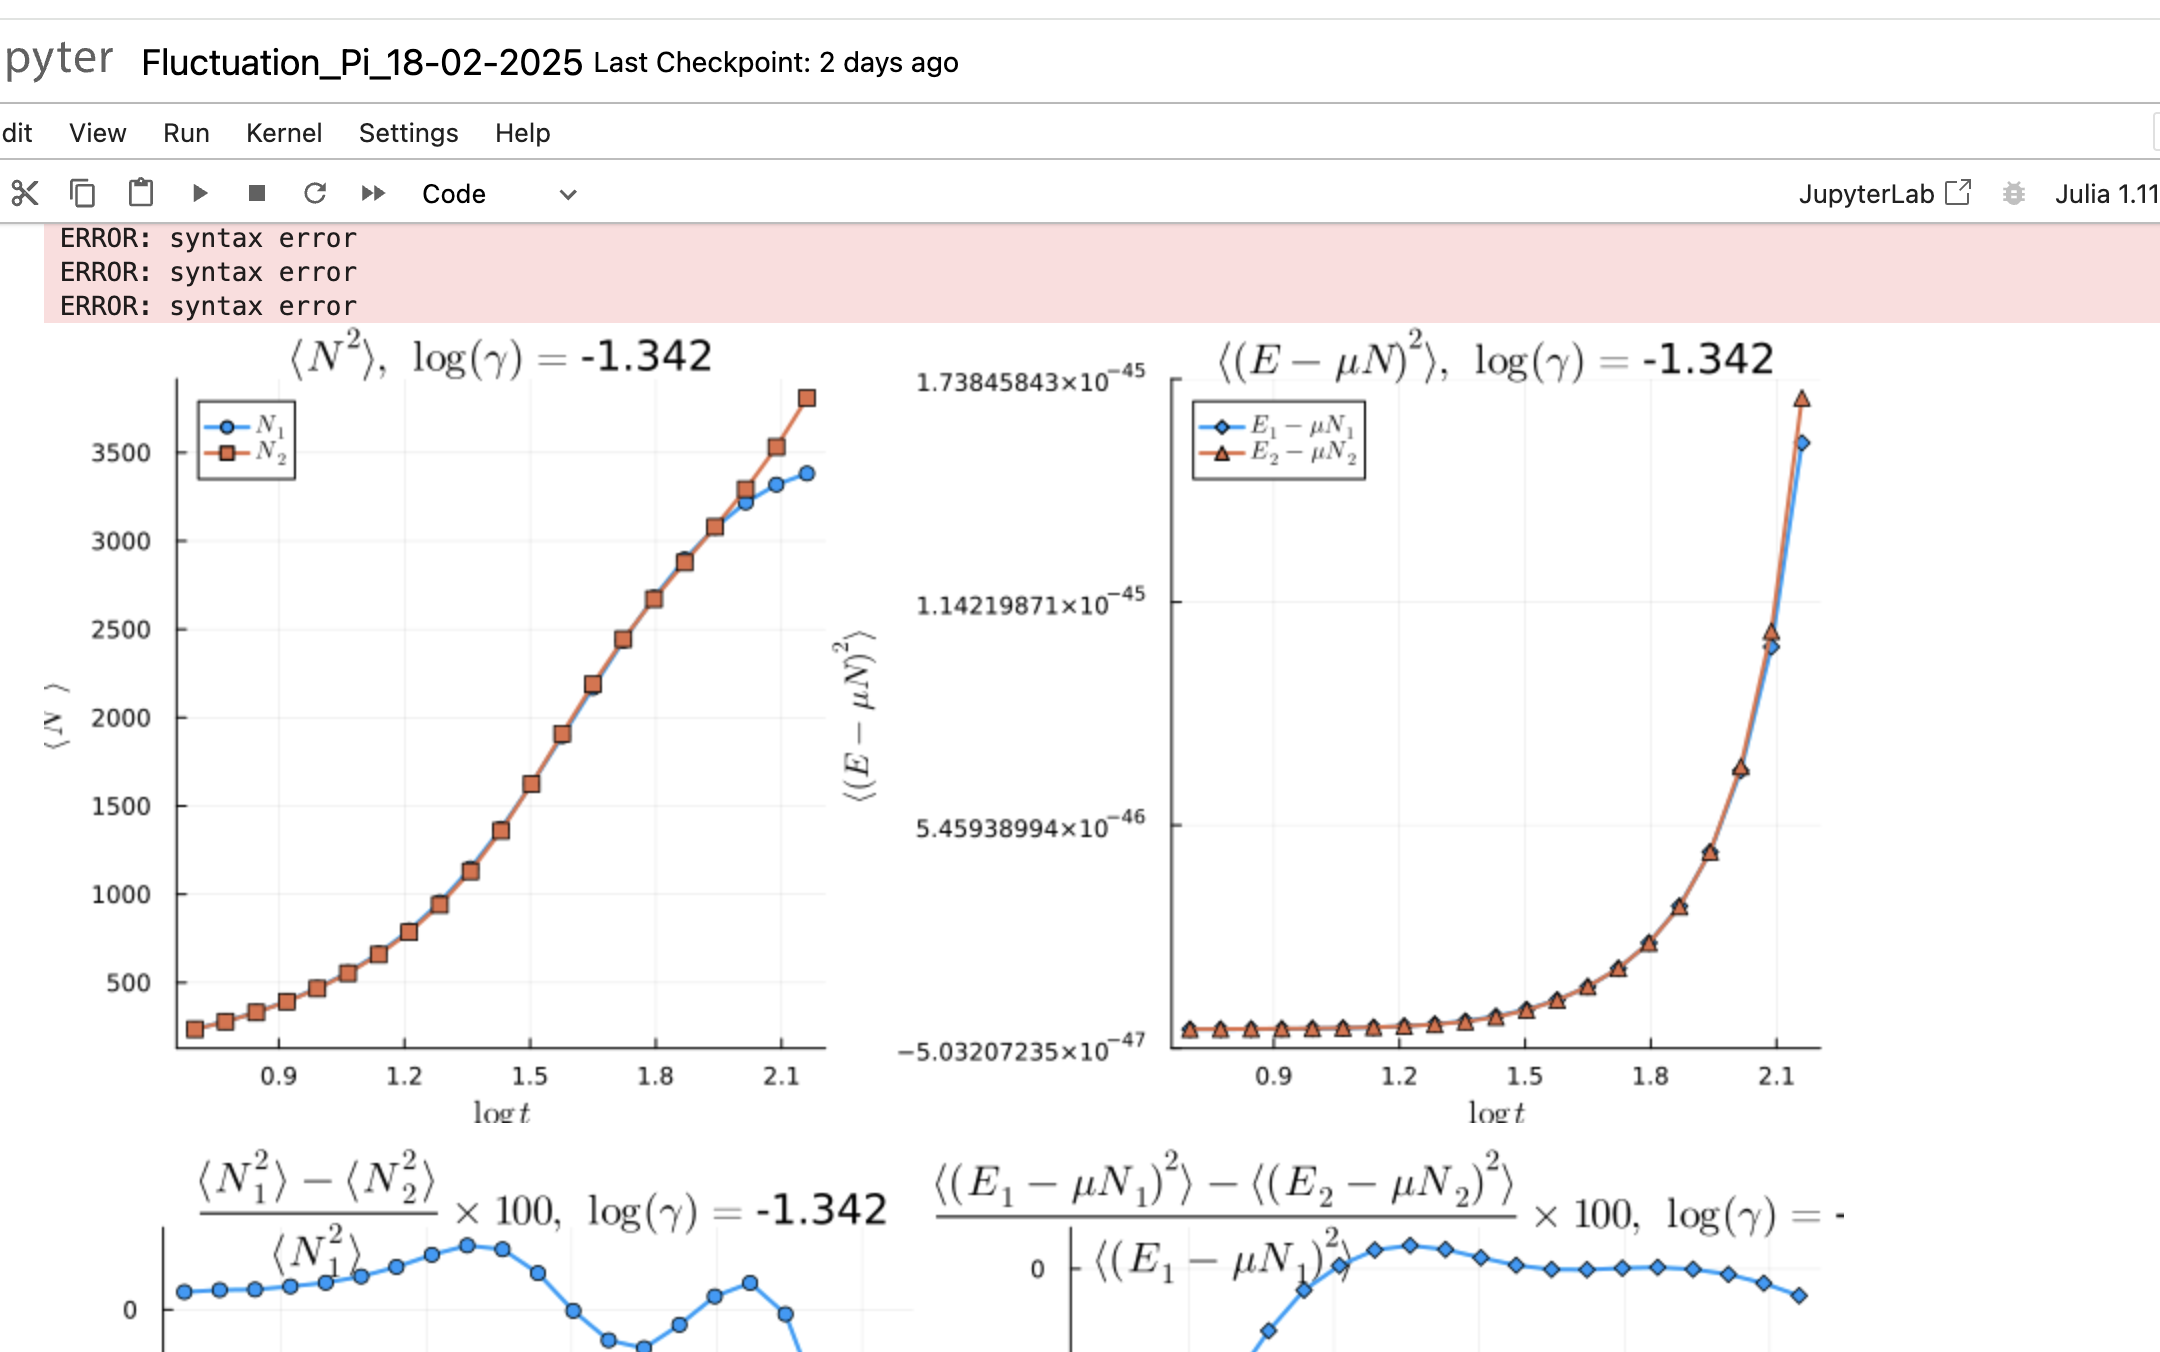
\includegraphics[width=1\textwidth]{Figures/test}

%\begin{aff}
%Donc une a l'ordre un en $\delta \theta (\operator{A}^{(0)})^{-1} %\operator{V}$ 

%\begin{eqnarray*}
%	\langle \delta \Pi ( \theta) \delta \Pi ( \theta') \rangle & = &  ( (\Pi^c_s - \Pi^c)\Pi^c/\Pi^c_s ) ( \theta ) \delta_{\theta, \theta'}/\delta \theta + \mathscr{F}(\theta , \theta' ) ,	
%\end{eqnarray*}

%avec 

%\begin{eqnarray*}
%	\mathscr{F}(\theta , \theta' ) & = & \left [ (\Pi^c_s - \Pi^c )( \theta)  +  (\Pi^c_s - \Pi^c ) ( \theta' )\right ] \frac{\Pi^c}{\Pi^c_s}(\theta)\frac{\Pi^c}{\Pi^c_s}(\theta') \frac{ \Delta( \theta'- \theta )}{ 2 \pi }\\
%	&&  - \left [ (\Pi^c_s - \Pi^c )( \theta)   (\Pi^c_s - \Pi^c ) ( \theta' )\right ] \frac{\Pi^c}{\Pi^c_s}(\theta)\frac{\Pi^c}{\Pi^c_s}(\theta')\int d\theta'' \left (   \frac{ \Pi^c/\Pi^c_s}{\Pi^c_s - \Pi^c} \right )(\theta'') \frac{\Delta(\theta''- \theta)}{2 \pi}\frac{\Delta(\theta''- \theta')}{2 \pi}  	
%\end{eqnarray*}
%\end{aff}



 








\subsection{Notion d’état d’équilibre généralisé (GGE)}

\paragraph{Introduction.}
Dans les systèmes quantiques intégrables, la dynamique unitaire à long temps ne conduit généralement pas à une thermalisation usuelle, au sens de l’ensemble canonique ou microcanonique. En effet, l'intégrabilité implique l'existence d'une infinité de charges conservées \( \operator{Q}_i \), en involution avec l’Hamiltonien \( \operator{H} \), i.e.
\begin{eqnarray*}
[\operator{Q}_i, \operator{H}] = 0,
\end{eqnarray*}
et entre elles : \( [\operator{Q}_i, \operator{Q}_j] = 0 \). Ces charges sont localement définies : chacune peut s’écrire sous la forme
\begin{eqnarray*}
\operator{Q}_i = \int dx\, \operator{q}_i(x),
\end{eqnarray*}
où \( \operator{q}_i(x) \) est une densité locale d’observable (ou "charge locale") à support fini. Cela signifie que pour tout \( i \), la densité \( \operator{q}_i(x) \) est une observable dont le support est contenu dans un sous-domaine borné de l’espace, noté \( \mathcal{S} \subset \mathbb{R} \).

Cette propriété de localité est essentielle pour décrire l’état du système à l’échelle mésoscopique ou dans un sous-système \( \mathcal{S} \), c’est-à-dire lorsque l’on restreint l’étude à une région finie du système total, typiquement après un processus de relaxation ou de déphasage local. Dans ce cas, le sous-système n’est pas décrit par un état thermique standard (de type Gibbs), mais par une distribution prenant en compte **l’ensemble des charges locales conservées** qui agissent effectivement dans la région \( \mathcal{S} \). Cette construction mène à la notion d’**état d’équilibre généralisé** ou **GGE** (pour *Generalized Gibbs Ensemble*).

L’état d’équilibre local généralisé est alors défini formellement par une matrice densité de la forme :
\begin{eqnarray*}
\operator{\rho}_{\mathcal{S}} = \frac{1}{Z_{\mathcal{S}}} \exp\left( -\sum_i \beta_i\, \operator{Q}_i^{(\mathcal{S})} \right),
\end{eqnarray*}
où \( \operator{Q}_i^{(\mathcal{S})} \) désigne la restriction de la charge \( \operator{Q}_i \) à la région \( \mathcal{S} \), c’est-à-dire :
\begin{eqnarray*}
\operator{Q}_i^{(\mathcal{S})} = \int_{\mathcal{S}} dx\, \operator{q}_i(x),
\end{eqnarray*}
et les coefficients \( \beta_i \in \mathbb{R} \) jouent le rôle de multiplicateurs de Lagrange associés à la conservation des \( \operator{Q}_i \) (on les interprète comme des "potentiels généralisés"). La constante \( Z_{\mathcal{S}} \) est le facteur de normalisation (ou "partition généralisée") :
\begin{eqnarray*}
Z_{\mathcal{S}} = \operatorname{Tr} \left[ \exp\left( -\sum_i \beta_i\, \operator{Q}_i^{(\mathcal{S})} \right) \right].
\end{eqnarray*}

Ce formalisme permet de décrire l’état macroscopique atteint par un système intégrable après relaxation unitaire, en particulier à la suite d’un *quench* quantique (changement soudain de paramètre). Contrairement à la situation standard où seule l’énergie est conservée, l’ensemble des charges \( \operator{Q}_i \) doit être pris en compte pour correctement prédire les observables locales dans l’état asymptotique.

L’approche GGE est donc un outil fondamental pour la description de l’équilibre local dans les systèmes intégrables, et permet notamment de comprendre pourquoi la thermalisation habituelle échoue dans ce contexte.

\paragraph{Configuration des états.}
On introduit la configuration $\{ \theta_a \}_{a\in \llbracket 1 , N_a \rrbracket} \equiv \{ \theta_1 , \cdots , \theta_{N_a} \}$ des rapidités pour un nombre $N_a$ de particules dépendant de la configuration $\{ \theta_a \}$  , et les états propres associés $\ket{\{ \theta_a \} }$.

%%%%%%%%%%%%%%%%%%%%%%%%%%%%%%%%%%%%%%%%%%%%%%%%%%
\paragraph{Observables diagonales dans la base des états propres.}
Dans le chapitre précédent (??), on a vu que l'état $\ket{\{ \theta_a \} }$ associé à cette configuration est une fonction propre des observables nombre et moment et  énergie (??). Ces observables sont diagonales dans la base des états propres :
\begin{eqnarray}
	\operator{Q}  =  \sum_{ \{\theta_a\} } \left ( \sum_{a = 1}^{N_a}  1 \right )  \vert \{ \theta_a\}\rangle	\langle \{ \theta_a \}\vert, \, 
	\operator{P}  =  \sum_{\{ \theta_a\}}\left( \sum_{a = 1}^{N_a}  \theta_a \right )   \vert \{ \theta_a\}\rangle	\langle \{ \theta_a \}\vert,\,\operator{H}  =  \sum_{\{ \theta_a\}}\left ( \sum_{a = 1}^{N_a} \frac{\theta_a^2}{2} \right )   \vert \{ \theta_a\}\rangle	\langle \{ \theta_a \}\vert.		
\end{eqnarray}

avec $ \sum_{\{ \theta_a\}}$ une somme sur tous les configurations.\\

%%%%%%%%%%%%%%%%%%%%%%%%%%%%%%%%%%%%%%%%%%%%
\paragraph{Contexte et GGE dans les systèmes intégrables.}

Dans un système quantique {\bf intégrable}, il existe une infinité de charges conservées locales $\operator{Q}_i$ commutant entre elles et avec l’Hamiltonien $\operator{H}$ ([Rigol et al. 2007] ). Concrètement, chaque charge se présente sous la forme $\operator{Q}_i = \int dx \,\operator{q}_i(x)$, où $\operator{q}_i(x)$ est une densité d’observable locale à support borné. L’intégrabilité implique ainsi une caractérisation complète des états propres par un ensemble de paramètres (rapidités $\{\theta_j\}$ dans le modèle de Lieb-Liniger). En particulier, contrairement aux systèmes génériques, un système intégrable ne thermalise pas au sens canonique classique, car la présence de toutes ces contraintes empêche l’oubli complet des conditions initiales. Les points clés sont alors :

\begin{itemize}[label = $\bullet$]
	\item {\bf Charges conservées} : infinité de locales $\operator{Q}_i$ satisfaisant et $[\operator{Q}_i , \operator{H} ] = 0$ et $[\operator{Q}_i , \operator{Q}_j ] = 0$.
	\item {\bf Densités locales} : chaque $\operator{Q}_i$ s’écrit $\operator{Q}_i = \int_\mathbb{R} dx \, \operator{q}_i(x)$ avec $\operator{q}_i(x)$ à support fini.
	\item {\bf Relaxation non canonique} : après un {\em quench} (changement brutal de paramètre), le système évolue vers un état stationnaire qui n’est pas décrit par l’ensemble canonique habituel.
\end{itemize}

Pour décrire cet état, on introduit l’{\bf ensemble de Gibbs généralisé (GGE)}. Rigol et al. ont montré qu’une « extension naturelle de l’ensemble de Gibbs aux systèmes intégrables » prédit correctement les valeurs moyennes des observables après relaxation.  Formellement, pour une région finie du système $\mathcal{S} \subset \mathbb{R}$, on définit la matrice densité locale :
\begin{eqnarray}
	\operator{\rho}^{(\mathcal{S})} = \frac{1}{Z^{(\mathcal{S})}}\exp \left ( - \sum_i \beta_i \operator{Q}_i^{(\mathcal{S})} \right), \quad \operator{Q}_i^{(\mathcal{S})} = \int_\mathcal{S} dx \, \operator{q}_i(x), 	
\end{eqnarray}

où $\beta_i \in \mathbb{R}$ sont les multiplicateurs de Lagrange (ou « températures généralisées ») associés aux charges locales conservées $\{\operator{Q}_i\}$. La fonction de partition $Z^{(\mathcal{S})} = \bm{\mathrm{Tr}}[\exp ( - \sum_i \beta_i \operator{Q}_i^{(\mathcal{S})} ) ]$ assure la normalisation. L’{\bf état GGE} ainsi défini est le seul permettant de prédire de manière cohérente les observables locales de $\mathcal{S}$ à long temps. Autrement dit, l’équilibre local après quench est un état stationnaire faisant perdurer la mémoire de chaque charge conservée, ce qui conduit à un nombre macroscopique de paramètres $\beta_i$ thermodynamiques (une « température » par charge).

 \subparagraph{Interprétation des multiplicateurs de Lagrange.}
Les multiplicateurs de Lagranges $\beta_i$ apparaissent naturellement lors de l'optimisation sous contraintes, par exemple dans le formalisme de l'{\bf ensemble de Gibbs généralisé (GGE)}, oû il imposent la conservation des valeurs moyennes des charges $\langle \operator{Q}_i^{(\mathcal{S})} \rangle_{\operator{\rho}^{(\mathcal{S})}} = \bm{\mathrm{Tr}}[\operator{\rho}^{(\mathcal{S})} \operator{Q}_i^{(\mathcal{S})}]   $.\\

En résumé, la GGE généralise les ensembles canoniques standard : au lieu de retenir uniquement l’énergie, on impose la conservation de l’ensemble complet $\{\operator{Q}_i \}$. Cette construction rend compte du fait que, dans un système intégrable, les observables locaux convergent vers les valeurs moyennes de , et non vers celles d’un Gibbs thermique ordinaire $\operator{\rho}^{(\mathcal{S})}$ . On comprend ainsi pourquoi la {\em thermalisation habituelle} (canonique ou microcanonique) échoue : seul l’ensemble de Gibbs généralisé peut intégrer toutes les contraintes locales.



%%%%%%%%%%%%%%%%%%%%%%%%%%%%%%%%%%%%%%%%%%%%%%%%%%
\paragraph{Charges conservées locales diagonales dans la base des états propres.}
Les charges conservées locales $\operator{Q}_i^{(\mathcal{S})}$ est diagonale dans la base des  états propres $\ket{ \{ \theta_a \}}$ , avec pour valeurs propres $\langle \operator{Q}_i^{(\mathcal{S})} \rangle_{\{\theta_a \}} = \bm{\mathrm{Tr}}[\ket{\{\theta_a \}}\!\bra{\{\theta_a \}} \operator{Q}_i^{(\mathcal{S})}] =  \bra{\{\theta_a \}} \operator{Q}_i^{(\mathcal{S})} \ket{\{\theta_a \}}$ :\\
\begin{eqnarray}
	\operator{Q}_i^{(\mathcal{S})} & = & \sum_{ \{\theta_a\} } \langle \operator{Q}_i^{(\mathcal{S})} \rangle_{\{\theta_a \}}  \ket{\{\theta_a \}}\!\bra{\{\theta_a \}}.		
\end{eqnarray}



%%%%%%%%%%%%%%%%%%%%%%%%%%%%%%%%%%%%%%%%
\paragraph{Probabilité d’un état à rapidités fixées.}
On peut alors définir la probabilité d’occurrence d’un état $\ket{\{ \theta_a \} }$ :
\begin{eqnarray}
	\mathbb{P}^{(\mathcal{S})} ( \{ \theta_a \} )  =  \bm{\mathrm{Tr}} \left [\operator{\rho}^{(\mathcal{S})} \ket{\{\theta_a \}}\!\bra{\{\theta_a \}} \right ] =  \bra{\{\theta_a \}}	\operator{\rho}^{(\mathcal{S})} \ket{\{\theta_a \}}  = \frac{1}{Z^{(\mathcal{S})}} \exp \left (- \sum_i \beta_i \langle \operator{Q}_i^{(\mathcal{S})} \rangle_{\{\theta_a \}} \right ) .
\end{eqnarray}

%%%%%%%%%%%%%%%%%%%%%%%%%%%
\paragraph{Moyenne d’un charges conservées locales et dérivées de $Z^{(\mathcal{S})}$.}
On peut écrire la moyenne d’une observable comme une somme pondérée par cette probabilité, ou encore comme une dérivée de la fonction de partition :
\begin{eqnarray}
	\langle \operator{Q}_i^{(\mathcal{S})} \rangle_{\operator{\rho}^{(\mathcal{S})}} &= & \sum_{\{ \theta_a\}} \langle \operator{Q}_i^{(\mathcal{S})} \rangle_{\{\theta_a \}} \mathbb{P}^{(\mathcal{S})} ( \{ \theta_a \} ) ~=~- \left. \frac{1}{Z^{(\mathcal{S})}} \frac{\partial Z^{(\mathcal{S})}}{\partial \beta_i} \right )_{\beta_{j \neq i }} ~=~ - 	\left . \frac{\partial  \ln Z^{(\mathcal{S})}}{\partial \beta_i} \right )_{\beta_{j \neq i }}	
\end{eqnarray}

Par le même raisonnement la moyenne de $(\operator{Q}_i^{(\mathcal{S})})^n$ s'écrit :

\begin{eqnarray}
	\langle (\operator{Q}_i^{(\mathcal{S})})^n \rangle &= & \sum_{\{ \theta_a\}} (\langle\operator{Q}_i^{(\mathcal{S})}\rangle_{\{\theta_a\}})^n \mathbb{P}^{(\mathcal{S})} ( \{ \theta_a \} ) ~=~ (-1)^n \left. \frac{1}{Z^{(\mathcal{S})}} \frac{\partial^n Z^{(\mathcal{S})}}{{(\partial \beta_i)}^n} \right )_{\beta_{j \neq i }} .	
\end{eqnarray}

%%%%%%%%%%%%%%%%%%%%%%%%%%%%%%%
\paragraph{Moments d’ordre supérieur et fluctuations.}
Le premier et second moments permettent d’accéder à la variance de l’observable :
\begin{eqnarray}
	\Delta_{\operator{Q}_i^{(\mathcal{S})}}^2 &=&  	\left \langle \left (\operator{Q}_i^{(\mathcal{S})} - \langle\operator{Q}_i^{(\mathcal{S})} \rangle_{\operator{\rho}^{(\mathcal{S})}} \right )^2  \right \rangle_{\operator{\rho}^{(\mathcal{S})}}  = 	\langle(\operator{Q}_i^{(\mathcal{S})})^2 \rangle_{\operator{\rho}^{(\mathcal{S})}}  -  \langle\operator{Q}_i^{(\mathcal{S})} \rangle_{\operator{\rho}^{(\mathcal{S})}}^2 \nonumber  \\
		& = & \left . \frac{1}{Z^{(\mathcal{S})}} \frac{ \partial^2 Z^{(\mathcal{S})} }{ {\partial \beta_i}^2 }  \right )_{\beta_{j\neq i}} - \left ( \left . \frac{1}{Z}\frac{ \partial Z^{(\mathcal{S})} }{ \partial \beta_i }  \right )_{\beta_{j\neq i}}\right )^2     \nonumber\\
		&=&  \frac{\partial}{\partial \beta_i } \left ( \left . \frac{1}{Z^{(\mathcal{S})}} \frac{\partial Z^{(\mathcal{S})}}{\partial \beta_i }  \right )_{\beta_{j\neq i}}  \right )_{\beta_{j\neq i}} \nonumber \\
		&=&	  \left . \frac{\partial^2 \ln Z^{(\mathcal{S})}  }{{\partial \beta_i}^2 }  \right )_{\beta_{j\neq i}} =  - \left . 	\frac{\partial \langle\operator{Q}_i^{(\mathcal{S})} \rangle_{\operator{\rho}^{(\mathcal{S})}} }{\partial \beta_i } \right )_{\beta_{j\neq i}}.	
\end{eqnarray}

%%%%%%%%%%%%%%%%%%%%%%%%%%%%%%
\paragraph{Cas particulier de l’équilibre thermique.}
-- Si $\operator{Q}_i^{(\mathcal{S})} = \operator{\mathcal{N}}$ alors $\beta_i = - \beta \mu $ et si $\operator{Q}_i^{(\mathcal{S})} = \operator{\mathcal{H}}_N - \mu \operator{\mathcal{N}} $ alors $\beta_i = \beta = T^{-1}$ (ici la constant de Boltzman $k_B = 1$) . Avec $\mu$ le potentielle chimique et $T$ la temperatures pour un équilibre thermique--.\\
Dans le cas d’un équilibre thermique, on identifie certains multiplicateurs à des grandeurs thermodynamiques classiques comme l’inverse de la température  et le potentiel chimique :	
\begin{eqnarray}
	\langle \operator{\mathcal{N}} \rangle_{\operator{\rho}^{(\mathcal{S})}}  = \left .\frac{1}{\beta} \frac{ \partial \ln Z^{(\mathcal{S})}}{\partial \mu } \right )_{T,\cdots},  & & \Delta^2_{\operator{\mathcal{N}}} = \left . \frac{1}{\beta^2} \frac{ \partial^2 \ln Z^{(\mathcal{S})}}{{\partial \mu}^2 } \right )_{T,\cdots} =  \left . \frac{1}{\beta} \frac{ \partial \langle \operator{\mathcal{N}} \rangle_{\operator{\rho}^{(\mathcal{S})}}}{\partial \mu } \right )_{T,\cdots}\\
	\langle \operator{\mathcal{H}}_N - \mu\operator{\mathcal{N}}  \rangle_{\operator{\rho}^{(\mathcal{S})}}  = -\left . \frac{ \partial \ln Z^{(\mathcal{S})}}{\partial \beta } \right )_{\mu , \cdots} ,  & & \Delta^2_{\operator{\mathcal{H}}_N - \mu\operator{\mathcal{N}}} = \left .  \frac{ \partial^2 \ln Z^{(\mathcal{S})}}{{\partial \beta}^2 } \right )_{\mu , \cdots} =  -\left .  \frac{ \partial \langle \operator{\mathcal{H}}_N - \mu\operator{\mathcal{N}} \rangle_{\operator{\rho}^{(\mathcal{S})}}}{\partial \beta } \right )_{\mu , \cdots}.		
\end{eqnarray}
Soit pour l'énergie, 
\begin{eqnarray}
	\langle \operator{\mathcal{H}}_N \rangle_{\operator{\rho}^{(\mathcal{S})}}  = \left [ \left .\frac{\mu}{\beta} \frac{ \partial}{\partial \mu } \right )_{T,\cdots} -\left . \frac{ \partial }{\partial \beta } \right )_\mu  \right ]\ln Z^{(\mathcal{S})},  \quad  \Delta^2_{\operator{\mathcal{H}}_N } = \left [ \left .\frac{\mu}{\beta} \frac{ \partial}{\partial \mu } \right )_{T,\cdots} -\left . \frac{ \partial }{\partial \beta } \right )_{\mu,\cdots}  \right ]^2\ln Z^{(\mathcal{S})}.		
\end{eqnarray}



%%Dans ce chapitre, nous nous intéressons aux fluctuations de la distribution de rapidité \( \delta \rho \) autour d'une distribution de référence \( \rho^c \), qui maximise la contribution à la fonction de partition des états, exprimée comme une fonctionnelle de la distribution \( \rho \) : 

La fonction de partition des états, s'exprime comme une fonctionnelle de la distribution \( \rho \) : 

\begin{eqnarray*}
	\Xi & = & \sum_\rho \exp \left( -\mathcal{A}(\rho) \right).
\end{eqnarray*}  

Dans la section {\em \bf Entropie de Yang-Yang} (\ref{??}), l'action \( \mathcal{A}(\rho) \) s'écrit sous la forme :  

\begin{eqnarray*}
	\mathcal{A}(\rho) & \doteq & - L\mathcal{S}_{YY}(\rho) + L\int f(\theta) \rho (\theta) \, d\theta,		
\end{eqnarray*}  

où \( \mathcal{S}_{YY} \) est la fonctionnelle d'entropie de Yang-Yang, définie dans (\ref{??}), et \( f \) est la fonction paramétrant les charges, introduite dans (\ref{??}).  

Dans cette même section {\em \bf Entropie de Yang-Yang} (\ref{??}), nous avons établi un lien entre \( f \) et distribution de référence \( \rho^c \), qui maximise la contribution à la fonction de partition des états .\\

On veux tester si nos experience est décrit pas un GGE. Pour cela nous nous intéressons aux fluctuations de la distribution de rapidité \( \delta \rho \) autour \( \rho^c \).

%Nous poursuivons à présent avec cette définition de l'action de classe $\mathcal{C}^2$ et admetant une distribution critique $\rho^c$ tel que sa différentielle en ce point critique soit nulle $d\mathcal{A}_{\rho^c} = 0 $ (\ref{??}) de sorte que d'aprés la formule de Taylor-Youg %afin de déterminer les fluctuations autour de \( \Pi^c \). Pour cela, nous réécrivons l'action sous la forme :  

Nous poursuivons à présent avec cette définition de l'action de classe $\mathcal{C}^2$ et admetant une distribution critique $\rho^c$ tel que sa différentielle en ce point critique soit nulle $d\mathcal{A}_{\rho^c} = 0 $ (\ref{??}) de sorte que d'aprés la formule de Taylor-Youg %afin de déterminer les fluctuations autour de \( \Pi^c \). Pour cela, nous réécrivons l'action sous la forme :  

\begin{eqnarray*}  
	\mathcal{A}(\rho^c + \delta \rho) & \underset{ \delta \rho \to 0 }{=} & \mathcal{A}(\rho^c)  + \frac{1}{2} \left. \frac{\delta^2 \mathcal{A}}{\delta \rho^2} \right|_{\rho^c} (\delta \rho) + \mathcal{O}((\delta \rho)^3),  
\end{eqnarray*}  

une expression quadratique pour l'action à l'ordre dominant en \( \delta \Pi \) avec $\left. \frac{\delta^2 \mathcal{A}}{\delta \rho^2} \right|_{\rho^c}$ la forme quadratique définie positive (Fig (\ref{fig.fluctu.A})).

\begin{figure}[H]
	\centering 
	\begin{tikzpicture}
		\begin{scope}[shift={(0,0)}]
			\begin{scope}[transform canvas={scale=0.6}]
				% Définition des couleurs avec les codes HTML
\definecolor{colorOne}{HTML}{443E46}
\definecolor{colorTwo}{HTML}{F6DEB8}
\definecolor{colorThree}{HTML}{908CA4}
\definecolor{colorFour}{HTML}{57659E}
\definecolor{colorFive}{HTML}{C57284}
\definecolor{colorSix}{HTML}{FF5B69}

% Raccourcis pour les couleurs
\def\colorOne{colorOne}
\def\colorTwo{colorTwo}
\def\colorThree{colorThree}
\def\colorFour{colorFour}
\def\colorFive{colorFive}
\def\colorSix{colorSix}

\def\colorslide{blue!50!black}



\begin{scope}
	% Tracer une courbe lisse entre des points
	\draw[shift={(0,0)} ,\colorOne]
		(-1 , 0 ) edge [thick,line width=0.8ex , ->,>=triangle 45  , \colorOne] node [pos = 1 , below ]{\huge$\rho$}( 5  , 0 )
	;
	\draw[shift={(0,0)}, color=\colorOne]
		(0, -1.0 ) edge [thick,line width=0.8ex , ->,>=triangle 45  ]node [pos=0.9,left=0.2cm ]{\huge$\mathcal{A}(\rho)$}( 0  , 5 )
	;
	\draw[]
		(2.5, 0.12 ) edge [thick,line width=0.8ex ,\colorThree ]node [pos=1,below  ]{\huge$\rho^c$} (2.5, -0.12 )	
	;
	
	\draw[]
		(2.5, -0.12 ) edge [thick,line width=0.4ex , dashed, \colorThree ] (2.5, 5.5 )
		(1.5, 1 ) edge [thick,line width=0.4ex , <->,>=triangle 45  , \colorThree ] (3.5, 1 )
		(-0.3,1) edge [thick,line width=0.4ex  , \colorThree ] node [pos=0,left ]{\huge$\mathcal{A}(\rho^c)$} (0.3, 1 )	
	;
    \draw[thick, line width=0.8ex , \colorFour] plot[smooth, tension=0.7] coordinates {
        (1, 5) (1.6 , 3 ) (2.5, 1) (3.5 , 3 )  (4, 5)
    };		
	
\end{scope}

	
			
			\end{scope}
			
			\draw[color = red , scale = 0.5 , draw = none  ] (-2 , -1) rectangle (5, 6) ; 	
		\end{scope}
		
		\begin{scope}[shift={(19,-1)}]
			\begin{scope}[transform canvas={scale=0.6}]
				% Définition des couleurs avec les codes HTML
\definecolor{colorOne}{HTML}{443E46}
\definecolor{colorTwo}{HTML}{F6DEB8}
\definecolor{colorThree}{HTML}{908CA4}
\definecolor{colorFour}{HTML}{57659E}
\definecolor{colorFive}{HTML}{C57284}
\definecolor{colorSix}{HTML}{FF5B69}

% Raccourcis pour les couleurs
\def\colorOne{colorOne}
\def\colorTwo{colorTwo}
\def\colorThree{colorThree}
\def\colorFour{colorFour}
\def\colorFive{colorFive}
\def\colorSix{colorSix}

\def\colorslide{blue!50!black}

\def\Occupation{
	\def\traitx{0.3}
	\def\traity{0.5}
	\draw[shift={(0,0)}]
		(-13.5 , 0 ) edge [thick,line width=0.8ex ]( -3.2  , 0 )
		( -3.2 - \traitx  , 0 - \traity ) edge [thick,line width=0.8ex ]( -3.2 + \traitx  , 0 + \traity  )
		( -2.8 - \traitx  , 0 - \traity ) edge [thick,line width=0.8ex ]( -2.8 + \traitx  , 0 + \traity  )
		(-2.8 , 0 ) edge [thick,line width=0.8ex ](2.8  , 0 )
		( 2.8 - \traitx  , 0 - \traity ) edge [thick,line width=0.8ex ]( 2.8 + \traitx  , 0 + \traity  )
		( 3.2 - \traitx  , 0 - \traity ) edge [thick,line width=0.8ex ]( 3.2 + \traitx  , 0 + \traity  )
		(3.2, 0 ) edge [thick,line width=0.8ex,->,>=triangle 45 , color = black ]node [pos=1.01,below  ]{\huge$\theta$}	( 13  , 0 )
	;
	\draw[shift={(0,0)}, color=\colorOne]
		(-10.5 , -1.5 ) edge [thick,line width=0.8ex , ->,>=triangle 45  ]( -10.5  , 4.5 )
	;
		
	\foreach \r in {1 , ... , 3 } {
%		\draw[
%		decoration={
%		markings,
%    	mark connection node=my node,
%    	mark=at position 0 with{\node [blue,transform shape] (my node) {\large \r};}},
%		color=gray, thick, 
%		line width=0.5ex] decorate { 
%            (-11.0, \r) -- (-10.1, \r )}
%        ;
        \draw[
			color=\colorOne,
			] 
            (-11.0, \r) edge[color=\colorThree , thick,line width=0.5ex] node [pos=-0.5 ]{\large\color{\colorFour} $\frac{\r}{\delta \theta}$ } (-10.3, \r )
        	;
	
	}
	

	
	% Graduation abcsisse 
	% Définitions des listes
% Definitions of the lists
\def\listetuple{-9/\theta_{1}, -8/\theta_{2} , -5/\theta_{3} , -2/\theta_{a-1} , 0/\theta_{a} , 1/\theta_{a+1} , 2/\theta_{a+2} ,  5/\theta_{N-4} , 7/\theta_{N-3},8/\theta_{N-1},9/\theta_{N} }
\def\listetrais{-12 , -11, -10, -9 , -8 , -7 ,  -6 , -5, -4.5,-4, -2 , -1, 0 , 0.5, 1, 2, 4 , 5 ,  6 , 7 , 8 ,8.5, 9 ,  10 , 11, 12 }

% Loop over listetrais
\foreach \r in \listetrais {
    % Initialize found variable to zero
    % Initialize found variable to zero
    %\pgfmathsetmacro\found{0}
    \global\def\found{0}
    \xdef\nomtheta{}
    
    % Check if \r is in listetuple
    \foreach \x/\y in \listetuple { 
        \ifdim \r pt=\x pt % If \r matches any \x in listetuple
            \global\def\found{1} ;
            \xdef\nomtheta{\y} % Set \nomtheta to the corresponding \y
            %\pgfmathsetmacro\found{1} % Set found to 1            
            %\global\pgfmathsetmacro\found{1}
        \fi
    }
    
    %\node [circle, draw, red] (A) at (\r, 2) {\found , $\nomtheta$};
    
    % Draw the line and display \nomtheta if found
    \ifnum\found=1
        \draw[color=\colorOne, thick, line width=0.5ex] 
            (\r, -0.3) -- (\r, 0.3) node[red , pos=-0.5] {\large $\nomtheta$};
         \filldraw[line width=0.5ex, color=\colorSix, outer color=\colorSix, inner color=\colorSix] 
            (\r, 0) circle (4pt);
    \else 
        % Draw without \nomtheta and add a blue circle if not found
        \draw[color=\colorOne, thick, line width=0.5ex] 
            (\r, -0.3) -- (\r, 0.3);
        \filldraw[line width=0.5ex, color=\colorSix, outer color=\colorTwo, inner color=\colorTwo] 
            (\r, 0) circle (4pt); 
    \fi
}

\def\listetrais{-9.5/\theta_{i-1}/2/3, -6.5/\theta_{i}/1/4  ,   -1.5/\theta_{j}/2/4 , 1.5/\theta_{j+1}/-1/3 , 3.5/\theta_{\ell-1}/1/3 , 6.5/\theta_{\ell}/3/4 , 9.5/\theta(\theta_{\ell+1})/-1/3 };



\foreach \r/\nomx/\y/\ys in \listetrais {
	\draw[
		decoration={
		markings,
    	mark connection node=my node,
    	mark=at position .5 with{\node [blue,transform shape] (my node) {\large \color{\colorFour} $\nomx$};}},
		color=\colorThree , thick, 
		line width=0.5ex] decorate { 
            (\r, 0.12) -- (\r, -1.2)}
        ;
     
     \ifdim \y pt > -1 pt 
     	\draw[
			decoration={
			markings,
    		mark connection node=my node,
    		mark=at position .5 with{\node [blue,transform shape] (my node) {\large \color{\colorFour} $\Pi(\nomx) $};}},
			color=\colorThree, thick, 
			line width=0.5ex] decorate { 
            (\r, \y) -- (\r +3, \y)}
        ;
        \draw[
			decoration={
			markings,
    		mark connection node=my node,
    		mark=at position .5 with{\node [blue,transform shape] (my node) {\large \color{\colorFive} $\Pi_s(\nomx) $};}},
			color=\colorFive, thick, 
			line width=0.5ex] decorate { 
            (\r, \ys) -- (\r +3, \ys)}
        ;
     \fi 
     \ifdim \r pt= -1.5 pt
     	\draw[
     		decoration={
			markings,
    		mark connection node=my node,
    		mark=at position .5 with{\node [blue,transform shape] (my node) {\large \color{\colorFour}  $\delta \theta $};},
    		%mark=at position 0.1  with {\arrow[blue, line width=0.5ex]{<}},
    		%mark=at position 1  with {\arrow[blue, line width=0.5ex]{>}}
    		},
        	color=\colorThree,
        	thick,
        	line width=0.5ex,
        	%arrows={Computer Modern Rightarrow[line cap=round]-Computer Modern Rightarrow[line cap=round]}
   			](\r, -1.2) edge[arrows={Computer Modern Rightarrow[line cap=round]-}] (\r + 0.4, -1.2)decorate {
    		(\r, -1.2) -- (\r + 3, -1.2)}(\r + 2, -1.2) edge[arrows={-Computer Modern Rightarrow[line cap=round]}] (\r + 3, -1.2)
    		;
    \fi
			
	
}


			
}


\begin{scope}
	%\draw[help lines , width=1.5ex] (-8,-3) grid (8,3);\draw[help lines ,width=0.5ex , opacity = 0.5] (-3,-3) grid[step=0.1] (3,3));
	
	%\draw[help lines] 
	%	(-3,-3) edge[width=1.5ex] grid (3,3)	
	%	(-3,-3) edge[width=0.5ex , opacity = 0.5] grid (3,3)	
	%;
	\begin{scope}[shift={(0,1)},rotate=0,opacity=1,color=black]
		\Occupation	
		
		%\node[anchor=east, font=\bfseries] at (-11, 0) {\color{red}\large (T = 0 )} ;	
	\end{scope}
	
	
	
	
	\begin{scope}[shift={(-10.5,7)},rotate=0,opacity=1,color=black]
	
	\begin{scope}[shift={(-0,0)},rotate=0,opacity=1,color=black]
	
		\draw[shift={(0,0)} ,line width=1ex,rounded corners = 1ex,color=\colorOne , opacity =1 ,fill=\colorOne!00 , pattern={north east lines} , pattern color=\colorOne!00 ]
			(0 , -1 ) rectangle (5,1)
		;
		

		\begin{scope}[shift={(0.5,0.5)}]
			\draw[color=\colorOne, thick, line width=0.5ex] 
            (0, -0.3) -- (0, 0.3) ;
            \filldraw[line width=0.5ex, color=\colorSix, outer color=\colorSix, inner color=\colorSix] 
            (0, 0) circle (4pt);
            
            \node[anchor=west, font=\bfseries] at (0.2, 0) {\color{\colorSix}\large : quasi-particule};
		\end{scope}
		
		\begin{scope}[shift={(0.5,-0.5)}]
			\draw[color=\colorOne, thick, line width=0.5ex] 
            (0, -0.3) -- (0, 0.3) ;
            \filldraw[line width=0.5ex, color=\colorSix, outer color=\colorTwo, inner color=\colorTwo] 
            (0, 0) circle (4pt);
            
            \node[anchor=west, font=\bfseries] at (0.2, 0) {\color{\colorSix}\large : hole};
		\end{scope}

	\end{scope}
	
	\begin{scope}[shift={(6,0)},rotate=0,opacity=1,color=black]	
		
		\draw[shift={(0,0)} ,line width=1ex,rounded corners = 1ex,color=\colorOne , opacity =1 ,fill=\colorOne!00 , pattern={north east lines} , pattern color=\colorOne!00 ]
			(0 , -1 ) rectangle (7.5,1)
		;
		
		\node[anchor=west] at (0.5, 0.5) {\color{\colorFour}\large $\Pi$ };\node[anchor=west, font=\bfseries] at (1, 0.5) {\color{\colorFour}\large : quasi-particule distribution};
		
		\node[anchor=west] at (0.5, -0.5) {\color{\colorFour}\large $\Pi_h$ };\node[anchor=west, font=\bfseries] at (1, -0.5) {\color{\colorFour}\large  : hole distribution};
		
	\end{scope}
	
	\begin{scope}[shift={(14.5,0)},rotate=0,opacity=1,color=black]	
		
		\draw[shift={(0,0)} ,line width=1ex,rounded corners = 1ex,color=\colorOne , opacity =1 ,fill=\colorOne!00 , pattern={north east lines} , pattern color=\colorOne!00 ]
			(0 , -0.5 ) rectangle (7.0,0.5)
		;
		
		\node[anchor=west] at (0.2, 0) {\color{\colorFour}\large ${\color{\colorFive}\Pi_s} = \Pi + \Pi_h $ } node[anchor=west , font=\bfseries] at (3.1 , 0 )  {\color{\colorFour}\large {\color{\colorFive} : density of states}};
		
	\end{scope}
	
	
	\end{scope}


		
	
\end{scope}

	
			
			\end{scope}
			\begin{scope}[scale=1]
				\draw[color = red , scale = 1 , draw = none  ] (-1 , -1) rectangle (5, 5) ; 
			\end{scope}	
		\end{scope}

		
				
			
	\end{tikzpicture}	
	\captionsetup{skip=10pt} % Ajoute de l’espace après la légende
	\label{fig.fluctu.A}
\end{figure}


On discrétise l'axe des rapidités en  petite cellule de rapidité $[\theta, \theta+\delta\theta]$, qui contient $L\rho(\theta) \delta \theta$ rapidités. 
	



Avec ces petites tranches, la forme quadratique s’écrit :

\begin{eqnarray*}
    \left. \frac{\delta^2 \mathcal{A}}{{\delta \rho}^2} \right|_{\rho^c}(\delta \rho ) &=&  \sum_{a,b \mid \text{tranche}}  
    \delta \rho(\theta_a)  \frac{\partial^2 \mathcal{A}}{\partial \delta \rho(\theta_a) \partial \delta \rho(\theta_b) } (\rho^c)  \delta \rho(\theta_b).
\end{eqnarray*}
Les fluctuations s’écrivent donc :

\begin{eqnarray*}
    \langle \delta \rho ( \theta) \delta \rho ( \theta') \rangle &=&  
    \frac{ \int d\delta \rho \, \delta \rho(\theta) \delta \rho ( \theta') 
    \exp \left( - \frac{1}{2} \sum_{a,b \mid \text{tranche}}  
    \delta \rho(\theta_a) \frac{\partial^2 \mathcal{A}}{\partial \delta \rho(\theta_a) \partial \delta \rho(\theta_b) } (\rho^c)  \delta \rho(\theta_b) \right) }
    { \int d\delta \Pi  
    \exp \left( - \frac{1}{2} \sum_{a,b \mid \text{tranche}}  
    \delta \rho(\theta_a) \frac{\partial^2 \mathcal{A}}{\partial \delta \rho(\theta_a) \partial \delta \rho(\theta_b) } (\rho^c)  \delta \rho(\theta_b) \right) } \\
    &=& \left( \mathbf{A}^{-1} \right)_{\theta , \theta'}
\end{eqnarray*}


\begin{aff}

\begin{eqnarray*}
	\langle \delta \rho ( \theta) \delta \rho ( \theta') \rangle &=& 	\left( \mathbf{A}^{-1} \right)_{\theta , \theta'}
\end{eqnarray*}

	
avec la  {\em matrice hessienne} $\mathbf{A}_{\theta , \theta'} \equiv \frac{\partial^2 \mathcal{A}}{\partial \delta \rho(\theta) \partial \delta \rho(\theta') }(\rho^c)$, au point critique/ qui maximise la probabilité  $\rho^c=\rho^c_s \nu^c $, s'écrit

\begin{eqnarray*}
	\operator{A} & = & \operator{A}^{(0)} + \delta \theta \operator{V}
\end{eqnarray*}

avec 

\begin{eqnarray*}
	A^{(0)}_{\theta , \theta'}  & = &  L\delta \theta \left ( \frac{ 1}{\rho^c_s ( 1  - \nu^c ) \nu^c } \right )(\theta)    \delta({\theta - \theta '})	,\\
	V_{\theta , \theta'}  &= & L \delta \theta \left \{ - \left [ \left ( \frac{1}{\rho^c_s( 1 - \nu^c) } \right ) ( \theta)  +  \left ( \frac{1}{\rho^c_s( 1 - \nu^c) } \right ) ( \theta' )\right ] \frac{ \Delta( \theta'- \theta )}{ 2 \pi } + \int d\theta''  \left ( \frac{\nu^c}{\rho^c_s( 1 - \nu^c) } \right )(\theta'') \frac{\Delta(\theta''- \theta)}{2 \pi}\frac{\Delta(\theta''- \theta')}{2 \pi}   \right \} 	
\end{eqnarray*}

\end{aff}

\subsection{Testes}

\begin{eqnarray*}
	\Delta_{\operator{\mathcal{N}}}^2  & = &  \frac{1}{\beta} \left . \frac{\partial \langle \operator{\mathcal{N}} \rangle}{\partial \mu} \right )_T \\
	\Delta_{\operator{\mathcal{E}}-\mu \operator{\mathcal{N}}}^2  & = &  - \left . \frac{\partial \langle \operator{\mathcal{E}}-\mu \operator{\mathcal{N}} \rangle}{\partial \beta} \right )_\mu 
\end{eqnarray*}

et 

\begin{eqnarray*}
	\Delta_{\operator{\mathcal{N}}}^2  &= & L^2 \int d\theta_a \int d \theta_b \, \langle \delta \rho(\theta_a) \delta \rho(\theta_b) \rangle \\
	\Delta_{\operator{\mathcal{E}}-\mu \operator{\mathcal{N}}}^2  & = & L^2 \int d\theta_a \int d \theta_b \, \left ( - \mu + \frac{1}2 m \theta_a^2  \right  )\left ( - \mu + \frac{1}2 m \theta_b^2  \right  )  \langle \delta \rho(\theta_a) \delta \rho(\theta_b) \rangle
\end{eqnarray*}

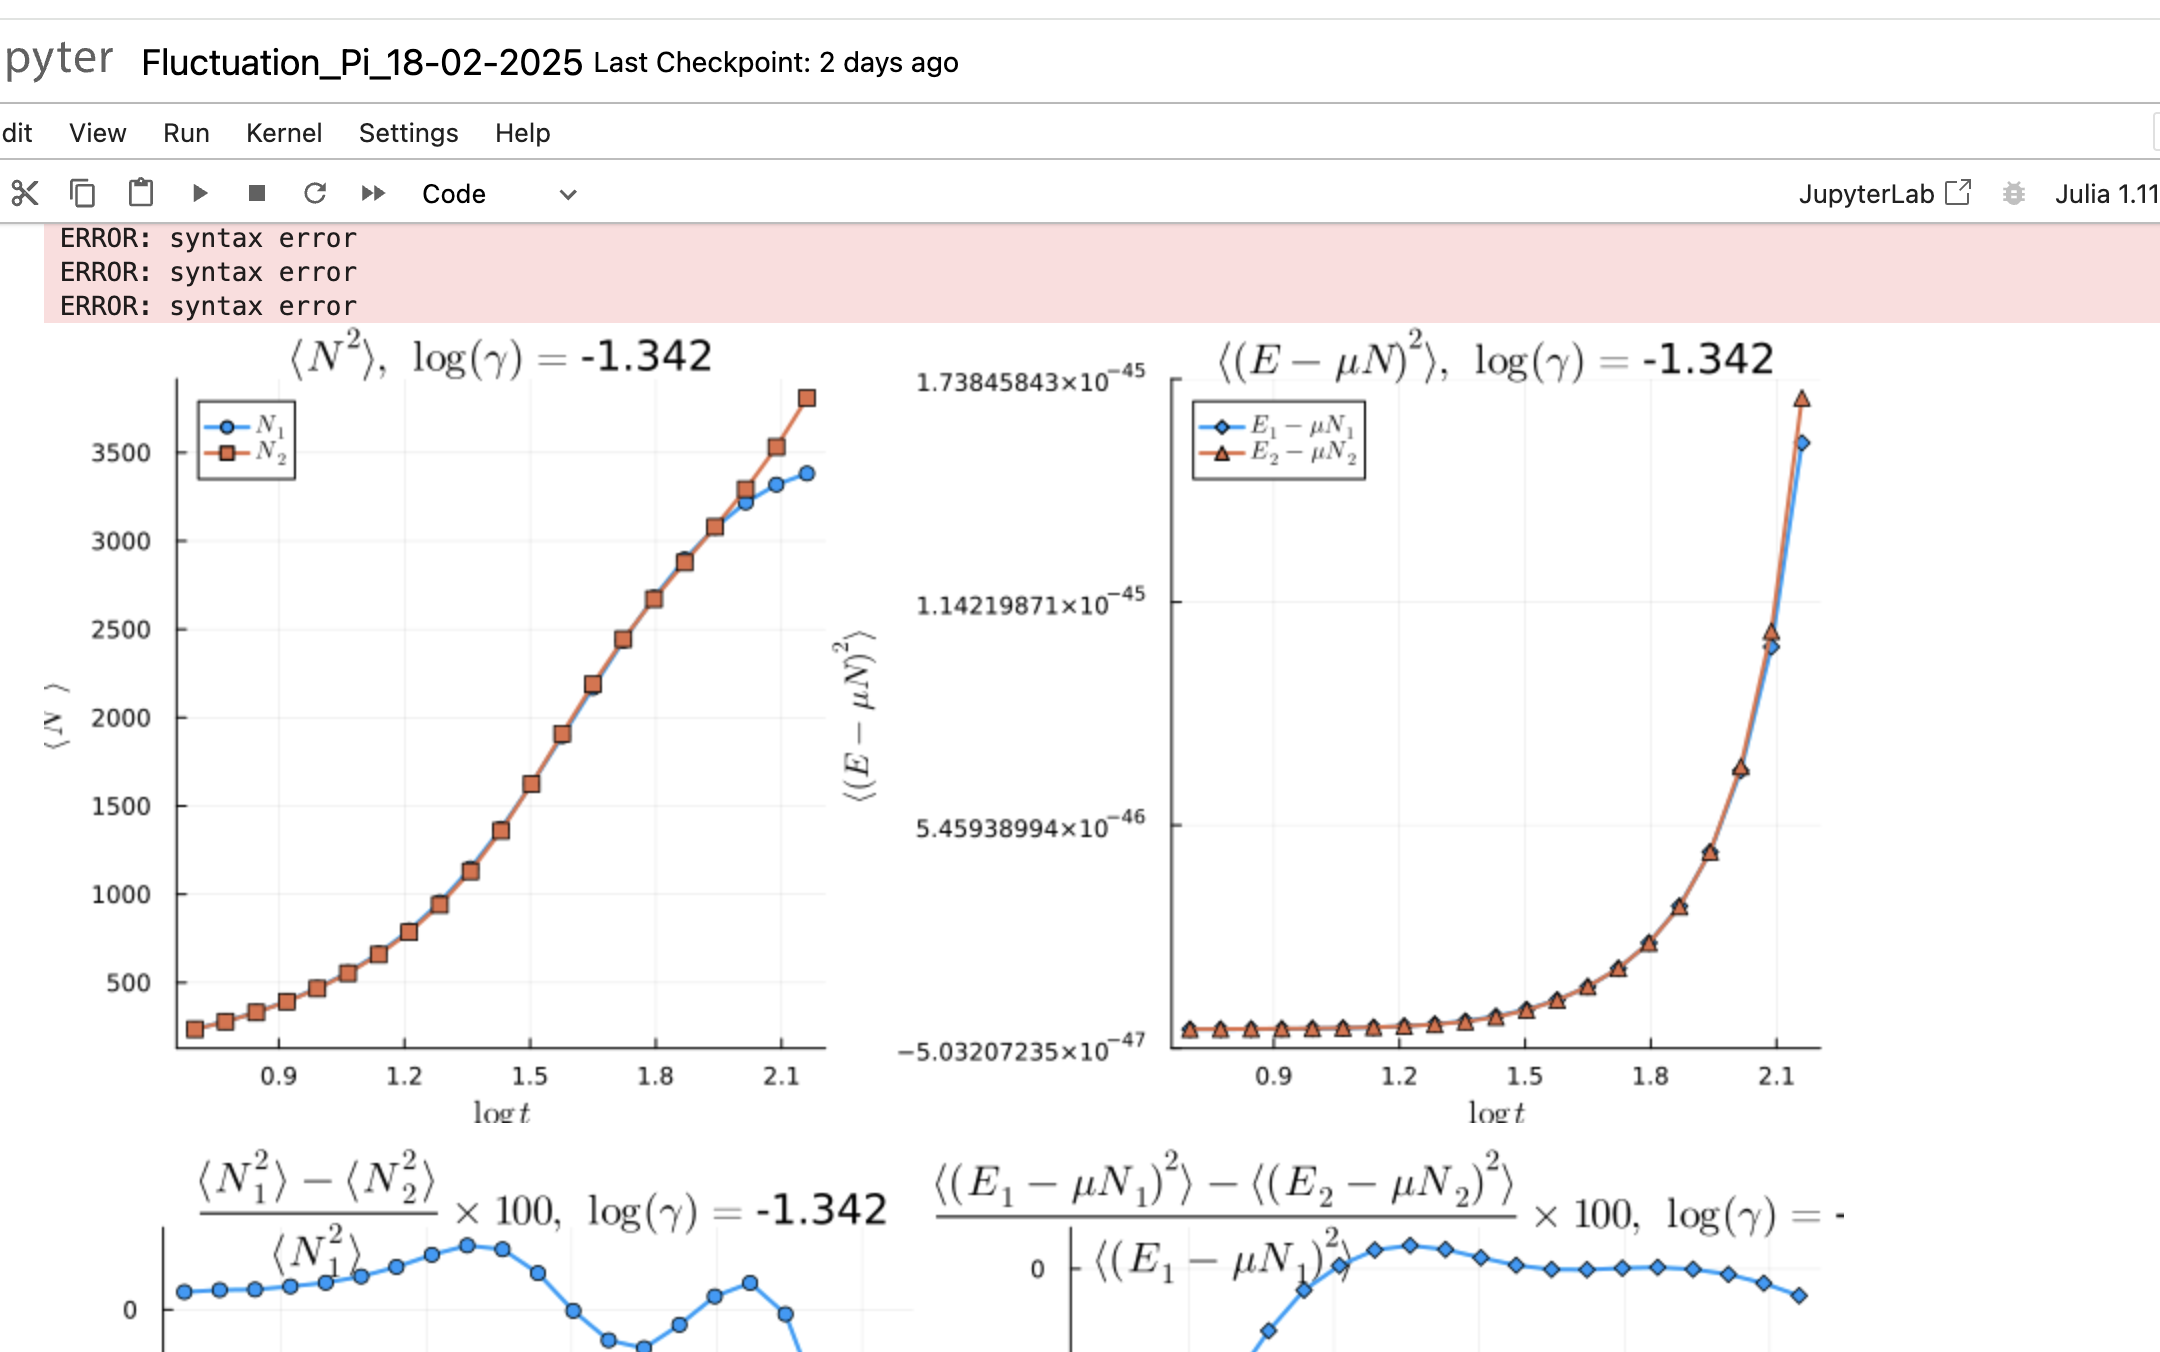
\includegraphics[width=1\textwidth]{Figures/test}

%\begin{aff}
%Donc une a l'ordre un en $\delta \theta (\operator{A}^{(0)})^{-1} %\operator{V}$ 

%\begin{eqnarray*}
%	\langle \delta \Pi ( \theta) \delta \Pi ( \theta') \rangle & = &  ( (\Pi^c_s - \Pi^c)\Pi^c/\Pi^c_s ) ( \theta ) \delta_{\theta, \theta'}/\delta \theta + \mathscr{F}(\theta , \theta' ) ,	
%\end{eqnarray*}

%avec 

%\begin{eqnarray*}
%	\mathscr{F}(\theta , \theta' ) & = & \left [ (\Pi^c_s - \Pi^c )( \theta)  +  (\Pi^c_s - \Pi^c ) ( \theta' )\right ] \frac{\Pi^c}{\Pi^c_s}(\theta)\frac{\Pi^c}{\Pi^c_s}(\theta') \frac{ \Delta( \theta'- \theta )}{ 2 \pi }\\
%	&&  - \left [ (\Pi^c_s - \Pi^c )( \theta)   (\Pi^c_s - \Pi^c ) ( \theta' )\right ] \frac{\Pi^c}{\Pi^c_s}(\theta)\frac{\Pi^c}{\Pi^c_s}(\theta')\int d\theta'' \left (   \frac{ \Pi^c/\Pi^c_s}{\Pi^c_s - \Pi^c} \right )(\theta'') \frac{\Delta(\theta''- \theta)}{2 \pi}\frac{\Delta(\theta''- \theta')}{2 \pi}  	
%\end{eqnarray*}
%\end{aff}



 








\subsection{Rôle des charges conservées extensives et quasi-locales}
%Dans ce chapitre, nous nous intéressons aux fluctuations de la distribution de rapidité \( \delta \rho \) autour d'une distribution de référence \( \rho^c \), qui maximise la contribution à la fonction de partition des états, exprimée comme une fonctionnelle de la distribution \( \rho \) : 

La fonction de partition des états, s'exprime comme une fonctionnelle de la distribution \( \rho \) : 

\begin{eqnarray*}
	\Xi & = & \sum_\rho \exp \left( -\mathcal{A}(\rho) \right).
\end{eqnarray*}  

Dans la section {\em \bf Entropie de Yang-Yang} (\ref{??}), l'action \( \mathcal{A}(\rho) \) s'écrit sous la forme :  

\begin{eqnarray*}
	\mathcal{A}(\rho) & \doteq & - L\mathcal{S}_{YY}(\rho) + L\int f(\theta) \rho (\theta) \, d\theta,		
\end{eqnarray*}  

où \( \mathcal{S}_{YY} \) est la fonctionnelle d'entropie de Yang-Yang, définie dans (\ref{??}), et \( f \) est la fonction paramétrant les charges, introduite dans (\ref{??}).  

Dans cette même section {\em \bf Entropie de Yang-Yang} (\ref{??}), nous avons établi un lien entre \( f \) et distribution de référence \( \rho^c \), qui maximise la contribution à la fonction de partition des états .\\

On veux tester si nos experience est décrit pas un GGE. Pour cela nous nous intéressons aux fluctuations de la distribution de rapidité \( \delta \rho \) autour \( \rho^c \).

%Nous poursuivons à présent avec cette définition de l'action de classe $\mathcal{C}^2$ et admetant une distribution critique $\rho^c$ tel que sa différentielle en ce point critique soit nulle $d\mathcal{A}_{\rho^c} = 0 $ (\ref{??}) de sorte que d'aprés la formule de Taylor-Youg %afin de déterminer les fluctuations autour de \( \Pi^c \). Pour cela, nous réécrivons l'action sous la forme :  

Nous poursuivons à présent avec cette définition de l'action de classe $\mathcal{C}^2$ et admetant une distribution critique $\rho^c$ tel que sa différentielle en ce point critique soit nulle $d\mathcal{A}_{\rho^c} = 0 $ (\ref{??}) de sorte que d'aprés la formule de Taylor-Youg %afin de déterminer les fluctuations autour de \( \Pi^c \). Pour cela, nous réécrivons l'action sous la forme :  

\begin{eqnarray*}  
	\mathcal{A}(\rho^c + \delta \rho) & \underset{ \delta \rho \to 0 }{=} & \mathcal{A}(\rho^c)  + \frac{1}{2} \left. \frac{\delta^2 \mathcal{A}}{\delta \rho^2} \right|_{\rho^c} (\delta \rho) + \mathcal{O}((\delta \rho)^3),  
\end{eqnarray*}  

une expression quadratique pour l'action à l'ordre dominant en \( \delta \Pi \) avec $\left. \frac{\delta^2 \mathcal{A}}{\delta \rho^2} \right|_{\rho^c}$ la forme quadratique définie positive (Fig (\ref{fig.fluctu.A})).

\begin{figure}[H]
	\centering 
	\begin{tikzpicture}
		\begin{scope}[shift={(0,0)}]
			\begin{scope}[transform canvas={scale=0.6}]
				% Définition des couleurs avec les codes HTML
\definecolor{colorOne}{HTML}{443E46}
\definecolor{colorTwo}{HTML}{F6DEB8}
\definecolor{colorThree}{HTML}{908CA4}
\definecolor{colorFour}{HTML}{57659E}
\definecolor{colorFive}{HTML}{C57284}
\definecolor{colorSix}{HTML}{FF5B69}

% Raccourcis pour les couleurs
\def\colorOne{colorOne}
\def\colorTwo{colorTwo}
\def\colorThree{colorThree}
\def\colorFour{colorFour}
\def\colorFive{colorFive}
\def\colorSix{colorSix}

\def\colorslide{blue!50!black}



\begin{scope}
	% Tracer une courbe lisse entre des points
	\draw[shift={(0,0)} ,\colorOne]
		(-1 , 0 ) edge [thick,line width=0.8ex , ->,>=triangle 45  , \colorOne] node [pos = 1 , below ]{\huge$\rho$}( 5  , 0 )
	;
	\draw[shift={(0,0)}, color=\colorOne]
		(0, -1.0 ) edge [thick,line width=0.8ex , ->,>=triangle 45  ]node [pos=0.9,left=0.2cm ]{\huge$\mathcal{A}(\rho)$}( 0  , 5 )
	;
	\draw[]
		(2.5, 0.12 ) edge [thick,line width=0.8ex ,\colorThree ]node [pos=1,below  ]{\huge$\rho^c$} (2.5, -0.12 )	
	;
	
	\draw[]
		(2.5, -0.12 ) edge [thick,line width=0.4ex , dashed, \colorThree ] (2.5, 5.5 )
		(1.5, 1 ) edge [thick,line width=0.4ex , <->,>=triangle 45  , \colorThree ] (3.5, 1 )
		(-0.3,1) edge [thick,line width=0.4ex  , \colorThree ] node [pos=0,left ]{\huge$\mathcal{A}(\rho^c)$} (0.3, 1 )	
	;
    \draw[thick, line width=0.8ex , \colorFour] plot[smooth, tension=0.7] coordinates {
        (1, 5) (1.6 , 3 ) (2.5, 1) (3.5 , 3 )  (4, 5)
    };		
	
\end{scope}

	
			
			\end{scope}
			
			\draw[color = red , scale = 0.5 , draw = none  ] (-2 , -1) rectangle (5, 6) ; 	
		\end{scope}
		
		\begin{scope}[shift={(19,-1)}]
			\begin{scope}[transform canvas={scale=0.6}]
				% Définition des couleurs avec les codes HTML
\definecolor{colorOne}{HTML}{443E46}
\definecolor{colorTwo}{HTML}{F6DEB8}
\definecolor{colorThree}{HTML}{908CA4}
\definecolor{colorFour}{HTML}{57659E}
\definecolor{colorFive}{HTML}{C57284}
\definecolor{colorSix}{HTML}{FF5B69}

% Raccourcis pour les couleurs
\def\colorOne{colorOne}
\def\colorTwo{colorTwo}
\def\colorThree{colorThree}
\def\colorFour{colorFour}
\def\colorFive{colorFive}
\def\colorSix{colorSix}

\def\colorslide{blue!50!black}

\def\Occupation{
	\def\traitx{0.3}
	\def\traity{0.5}
	\draw[shift={(0,0)}]
		(-13.5 , 0 ) edge [thick,line width=0.8ex ]( -3.2  , 0 )
		( -3.2 - \traitx  , 0 - \traity ) edge [thick,line width=0.8ex ]( -3.2 + \traitx  , 0 + \traity  )
		( -2.8 - \traitx  , 0 - \traity ) edge [thick,line width=0.8ex ]( -2.8 + \traitx  , 0 + \traity  )
		(-2.8 , 0 ) edge [thick,line width=0.8ex ](2.8  , 0 )
		( 2.8 - \traitx  , 0 - \traity ) edge [thick,line width=0.8ex ]( 2.8 + \traitx  , 0 + \traity  )
		( 3.2 - \traitx  , 0 - \traity ) edge [thick,line width=0.8ex ]( 3.2 + \traitx  , 0 + \traity  )
		(3.2, 0 ) edge [thick,line width=0.8ex,->,>=triangle 45 , color = black ]node [pos=1.01,below  ]{\huge$\theta$}	( 13  , 0 )
	;
	\draw[shift={(0,0)}, color=\colorOne]
		(-10.5 , -1.5 ) edge [thick,line width=0.8ex , ->,>=triangle 45  ]( -10.5  , 4.5 )
	;
		
	\foreach \r in {1 , ... , 3 } {
%		\draw[
%		decoration={
%		markings,
%    	mark connection node=my node,
%    	mark=at position 0 with{\node [blue,transform shape] (my node) {\large \r};}},
%		color=gray, thick, 
%		line width=0.5ex] decorate { 
%            (-11.0, \r) -- (-10.1, \r )}
%        ;
        \draw[
			color=\colorOne,
			] 
            (-11.0, \r) edge[color=\colorThree , thick,line width=0.5ex] node [pos=-0.5 ]{\large\color{\colorFour} $\frac{\r}{\delta \theta}$ } (-10.3, \r )
        	;
	
	}
	

	
	% Graduation abcsisse 
	% Définitions des listes
% Definitions of the lists
\def\listetuple{-9/\theta_{1}, -8/\theta_{2} , -5/\theta_{3} , -2/\theta_{a-1} , 0/\theta_{a} , 1/\theta_{a+1} , 2/\theta_{a+2} ,  5/\theta_{N-4} , 7/\theta_{N-3},8/\theta_{N-1},9/\theta_{N} }
\def\listetrais{-12 , -11, -10, -9 , -8 , -7 ,  -6 , -5, -4.5,-4, -2 , -1, 0 , 0.5, 1, 2, 4 , 5 ,  6 , 7 , 8 ,8.5, 9 ,  10 , 11, 12 }

% Loop over listetrais
\foreach \r in \listetrais {
    % Initialize found variable to zero
    % Initialize found variable to zero
    %\pgfmathsetmacro\found{0}
    \global\def\found{0}
    \xdef\nomtheta{}
    
    % Check if \r is in listetuple
    \foreach \x/\y in \listetuple { 
        \ifdim \r pt=\x pt % If \r matches any \x in listetuple
            \global\def\found{1} ;
            \xdef\nomtheta{\y} % Set \nomtheta to the corresponding \y
            %\pgfmathsetmacro\found{1} % Set found to 1            
            %\global\pgfmathsetmacro\found{1}
        \fi
    }
    
    %\node [circle, draw, red] (A) at (\r, 2) {\found , $\nomtheta$};
    
    % Draw the line and display \nomtheta if found
    \ifnum\found=1
        \draw[color=\colorOne, thick, line width=0.5ex] 
            (\r, -0.3) -- (\r, 0.3) node[red , pos=-0.5] {\large $\nomtheta$};
         \filldraw[line width=0.5ex, color=\colorSix, outer color=\colorSix, inner color=\colorSix] 
            (\r, 0) circle (4pt);
    \else 
        % Draw without \nomtheta and add a blue circle if not found
        \draw[color=\colorOne, thick, line width=0.5ex] 
            (\r, -0.3) -- (\r, 0.3);
        \filldraw[line width=0.5ex, color=\colorSix, outer color=\colorTwo, inner color=\colorTwo] 
            (\r, 0) circle (4pt); 
    \fi
}

\def\listetrais{-9.5/\theta_{i-1}/2/3, -6.5/\theta_{i}/1/4  ,   -1.5/\theta_{j}/2/4 , 1.5/\theta_{j+1}/-1/3 , 3.5/\theta_{\ell-1}/1/3 , 6.5/\theta_{\ell}/3/4 , 9.5/\theta(\theta_{\ell+1})/-1/3 };



\foreach \r/\nomx/\y/\ys in \listetrais {
	\draw[
		decoration={
		markings,
    	mark connection node=my node,
    	mark=at position .5 with{\node [blue,transform shape] (my node) {\large \color{\colorFour} $\nomx$};}},
		color=\colorThree , thick, 
		line width=0.5ex] decorate { 
            (\r, 0.12) -- (\r, -1.2)}
        ;
     
     \ifdim \y pt > -1 pt 
     	\draw[
			decoration={
			markings,
    		mark connection node=my node,
    		mark=at position .5 with{\node [blue,transform shape] (my node) {\large \color{\colorFour} $\Pi(\nomx) $};}},
			color=\colorThree, thick, 
			line width=0.5ex] decorate { 
            (\r, \y) -- (\r +3, \y)}
        ;
        \draw[
			decoration={
			markings,
    		mark connection node=my node,
    		mark=at position .5 with{\node [blue,transform shape] (my node) {\large \color{\colorFive} $\Pi_s(\nomx) $};}},
			color=\colorFive, thick, 
			line width=0.5ex] decorate { 
            (\r, \ys) -- (\r +3, \ys)}
        ;
     \fi 
     \ifdim \r pt= -1.5 pt
     	\draw[
     		decoration={
			markings,
    		mark connection node=my node,
    		mark=at position .5 with{\node [blue,transform shape] (my node) {\large \color{\colorFour}  $\delta \theta $};},
    		%mark=at position 0.1  with {\arrow[blue, line width=0.5ex]{<}},
    		%mark=at position 1  with {\arrow[blue, line width=0.5ex]{>}}
    		},
        	color=\colorThree,
        	thick,
        	line width=0.5ex,
        	%arrows={Computer Modern Rightarrow[line cap=round]-Computer Modern Rightarrow[line cap=round]}
   			](\r, -1.2) edge[arrows={Computer Modern Rightarrow[line cap=round]-}] (\r + 0.4, -1.2)decorate {
    		(\r, -1.2) -- (\r + 3, -1.2)}(\r + 2, -1.2) edge[arrows={-Computer Modern Rightarrow[line cap=round]}] (\r + 3, -1.2)
    		;
    \fi
			
	
}


			
}


\begin{scope}
	%\draw[help lines , width=1.5ex] (-8,-3) grid (8,3);\draw[help lines ,width=0.5ex , opacity = 0.5] (-3,-3) grid[step=0.1] (3,3));
	
	%\draw[help lines] 
	%	(-3,-3) edge[width=1.5ex] grid (3,3)	
	%	(-3,-3) edge[width=0.5ex , opacity = 0.5] grid (3,3)	
	%;
	\begin{scope}[shift={(0,1)},rotate=0,opacity=1,color=black]
		\Occupation	
		
		%\node[anchor=east, font=\bfseries] at (-11, 0) {\color{red}\large (T = 0 )} ;	
	\end{scope}
	
	
	
	
	\begin{scope}[shift={(-10.5,7)},rotate=0,opacity=1,color=black]
	
	\begin{scope}[shift={(-0,0)},rotate=0,opacity=1,color=black]
	
		\draw[shift={(0,0)} ,line width=1ex,rounded corners = 1ex,color=\colorOne , opacity =1 ,fill=\colorOne!00 , pattern={north east lines} , pattern color=\colorOne!00 ]
			(0 , -1 ) rectangle (5,1)
		;
		

		\begin{scope}[shift={(0.5,0.5)}]
			\draw[color=\colorOne, thick, line width=0.5ex] 
            (0, -0.3) -- (0, 0.3) ;
            \filldraw[line width=0.5ex, color=\colorSix, outer color=\colorSix, inner color=\colorSix] 
            (0, 0) circle (4pt);
            
            \node[anchor=west, font=\bfseries] at (0.2, 0) {\color{\colorSix}\large : quasi-particule};
		\end{scope}
		
		\begin{scope}[shift={(0.5,-0.5)}]
			\draw[color=\colorOne, thick, line width=0.5ex] 
            (0, -0.3) -- (0, 0.3) ;
            \filldraw[line width=0.5ex, color=\colorSix, outer color=\colorTwo, inner color=\colorTwo] 
            (0, 0) circle (4pt);
            
            \node[anchor=west, font=\bfseries] at (0.2, 0) {\color{\colorSix}\large : hole};
		\end{scope}

	\end{scope}
	
	\begin{scope}[shift={(6,0)},rotate=0,opacity=1,color=black]	
		
		\draw[shift={(0,0)} ,line width=1ex,rounded corners = 1ex,color=\colorOne , opacity =1 ,fill=\colorOne!00 , pattern={north east lines} , pattern color=\colorOne!00 ]
			(0 , -1 ) rectangle (7.5,1)
		;
		
		\node[anchor=west] at (0.5, 0.5) {\color{\colorFour}\large $\Pi$ };\node[anchor=west, font=\bfseries] at (1, 0.5) {\color{\colorFour}\large : quasi-particule distribution};
		
		\node[anchor=west] at (0.5, -0.5) {\color{\colorFour}\large $\Pi_h$ };\node[anchor=west, font=\bfseries] at (1, -0.5) {\color{\colorFour}\large  : hole distribution};
		
	\end{scope}
	
	\begin{scope}[shift={(14.5,0)},rotate=0,opacity=1,color=black]	
		
		\draw[shift={(0,0)} ,line width=1ex,rounded corners = 1ex,color=\colorOne , opacity =1 ,fill=\colorOne!00 , pattern={north east lines} , pattern color=\colorOne!00 ]
			(0 , -0.5 ) rectangle (7.0,0.5)
		;
		
		\node[anchor=west] at (0.2, 0) {\color{\colorFour}\large ${\color{\colorFive}\Pi_s} = \Pi + \Pi_h $ } node[anchor=west , font=\bfseries] at (3.1 , 0 )  {\color{\colorFour}\large {\color{\colorFive} : density of states}};
		
	\end{scope}
	
	
	\end{scope}


		
	
\end{scope}

	
			
			\end{scope}
			\begin{scope}[scale=1]
				\draw[color = red , scale = 1 , draw = none  ] (-1 , -1) rectangle (5, 5) ; 
			\end{scope}	
		\end{scope}

		
				
			
	\end{tikzpicture}	
	\captionsetup{skip=10pt} % Ajoute de l’espace après la légende
	\label{fig.fluctu.A}
\end{figure}


On discrétise l'axe des rapidités en  petite cellule de rapidité $[\theta, \theta+\delta\theta]$, qui contient $L\rho(\theta) \delta \theta$ rapidités. 
	



Avec ces petites tranches, la forme quadratique s’écrit :

\begin{eqnarray*}
    \left. \frac{\delta^2 \mathcal{A}}{{\delta \rho}^2} \right|_{\rho^c}(\delta \rho ) &=&  \sum_{a,b \mid \text{tranche}}  
    \delta \rho(\theta_a)  \frac{\partial^2 \mathcal{A}}{\partial \delta \rho(\theta_a) \partial \delta \rho(\theta_b) } (\rho^c)  \delta \rho(\theta_b).
\end{eqnarray*}
Les fluctuations s’écrivent donc :

\begin{eqnarray*}
    \langle \delta \rho ( \theta) \delta \rho ( \theta') \rangle &=&  
    \frac{ \int d\delta \rho \, \delta \rho(\theta) \delta \rho ( \theta') 
    \exp \left( - \frac{1}{2} \sum_{a,b \mid \text{tranche}}  
    \delta \rho(\theta_a) \frac{\partial^2 \mathcal{A}}{\partial \delta \rho(\theta_a) \partial \delta \rho(\theta_b) } (\rho^c)  \delta \rho(\theta_b) \right) }
    { \int d\delta \Pi  
    \exp \left( - \frac{1}{2} \sum_{a,b \mid \text{tranche}}  
    \delta \rho(\theta_a) \frac{\partial^2 \mathcal{A}}{\partial \delta \rho(\theta_a) \partial \delta \rho(\theta_b) } (\rho^c)  \delta \rho(\theta_b) \right) } \\
    &=& \left( \mathbf{A}^{-1} \right)_{\theta , \theta'}
\end{eqnarray*}


\begin{aff}

\begin{eqnarray*}
	\langle \delta \rho ( \theta) \delta \rho ( \theta') \rangle &=& 	\left( \mathbf{A}^{-1} \right)_{\theta , \theta'}
\end{eqnarray*}

	
avec la  {\em matrice hessienne} $\mathbf{A}_{\theta , \theta'} \equiv \frac{\partial^2 \mathcal{A}}{\partial \delta \rho(\theta) \partial \delta \rho(\theta') }(\rho^c)$, au point critique/ qui maximise la probabilité  $\rho^c=\rho^c_s \nu^c $, s'écrit

\begin{eqnarray*}
	\operator{A} & = & \operator{A}^{(0)} + \delta \theta \operator{V}
\end{eqnarray*}

avec 

\begin{eqnarray*}
	A^{(0)}_{\theta , \theta'}  & = &  L\delta \theta \left ( \frac{ 1}{\rho^c_s ( 1  - \nu^c ) \nu^c } \right )(\theta)    \delta({\theta - \theta '})	,\\
	V_{\theta , \theta'}  &= & L \delta \theta \left \{ - \left [ \left ( \frac{1}{\rho^c_s( 1 - \nu^c) } \right ) ( \theta)  +  \left ( \frac{1}{\rho^c_s( 1 - \nu^c) } \right ) ( \theta' )\right ] \frac{ \Delta( \theta'- \theta )}{ 2 \pi } + \int d\theta''  \left ( \frac{\nu^c}{\rho^c_s( 1 - \nu^c) } \right )(\theta'') \frac{\Delta(\theta''- \theta)}{2 \pi}\frac{\Delta(\theta''- \theta')}{2 \pi}   \right \} 	
\end{eqnarray*}

\end{aff}

\subsection{Testes}

\begin{eqnarray*}
	\Delta_{\operator{\mathcal{N}}}^2  & = &  \frac{1}{\beta} \left . \frac{\partial \langle \operator{\mathcal{N}} \rangle}{\partial \mu} \right )_T \\
	\Delta_{\operator{\mathcal{E}}-\mu \operator{\mathcal{N}}}^2  & = &  - \left . \frac{\partial \langle \operator{\mathcal{E}}-\mu \operator{\mathcal{N}} \rangle}{\partial \beta} \right )_\mu 
\end{eqnarray*}

et 

\begin{eqnarray*}
	\Delta_{\operator{\mathcal{N}}}^2  &= & L^2 \int d\theta_a \int d \theta_b \, \langle \delta \rho(\theta_a) \delta \rho(\theta_b) \rangle \\
	\Delta_{\operator{\mathcal{E}}-\mu \operator{\mathcal{N}}}^2  & = & L^2 \int d\theta_a \int d \theta_b \, \left ( - \mu + \frac{1}2 m \theta_a^2  \right  )\left ( - \mu + \frac{1}2 m \theta_b^2  \right  )  \langle \delta \rho(\theta_a) \delta \rho(\theta_b) \rangle
\end{eqnarray*}

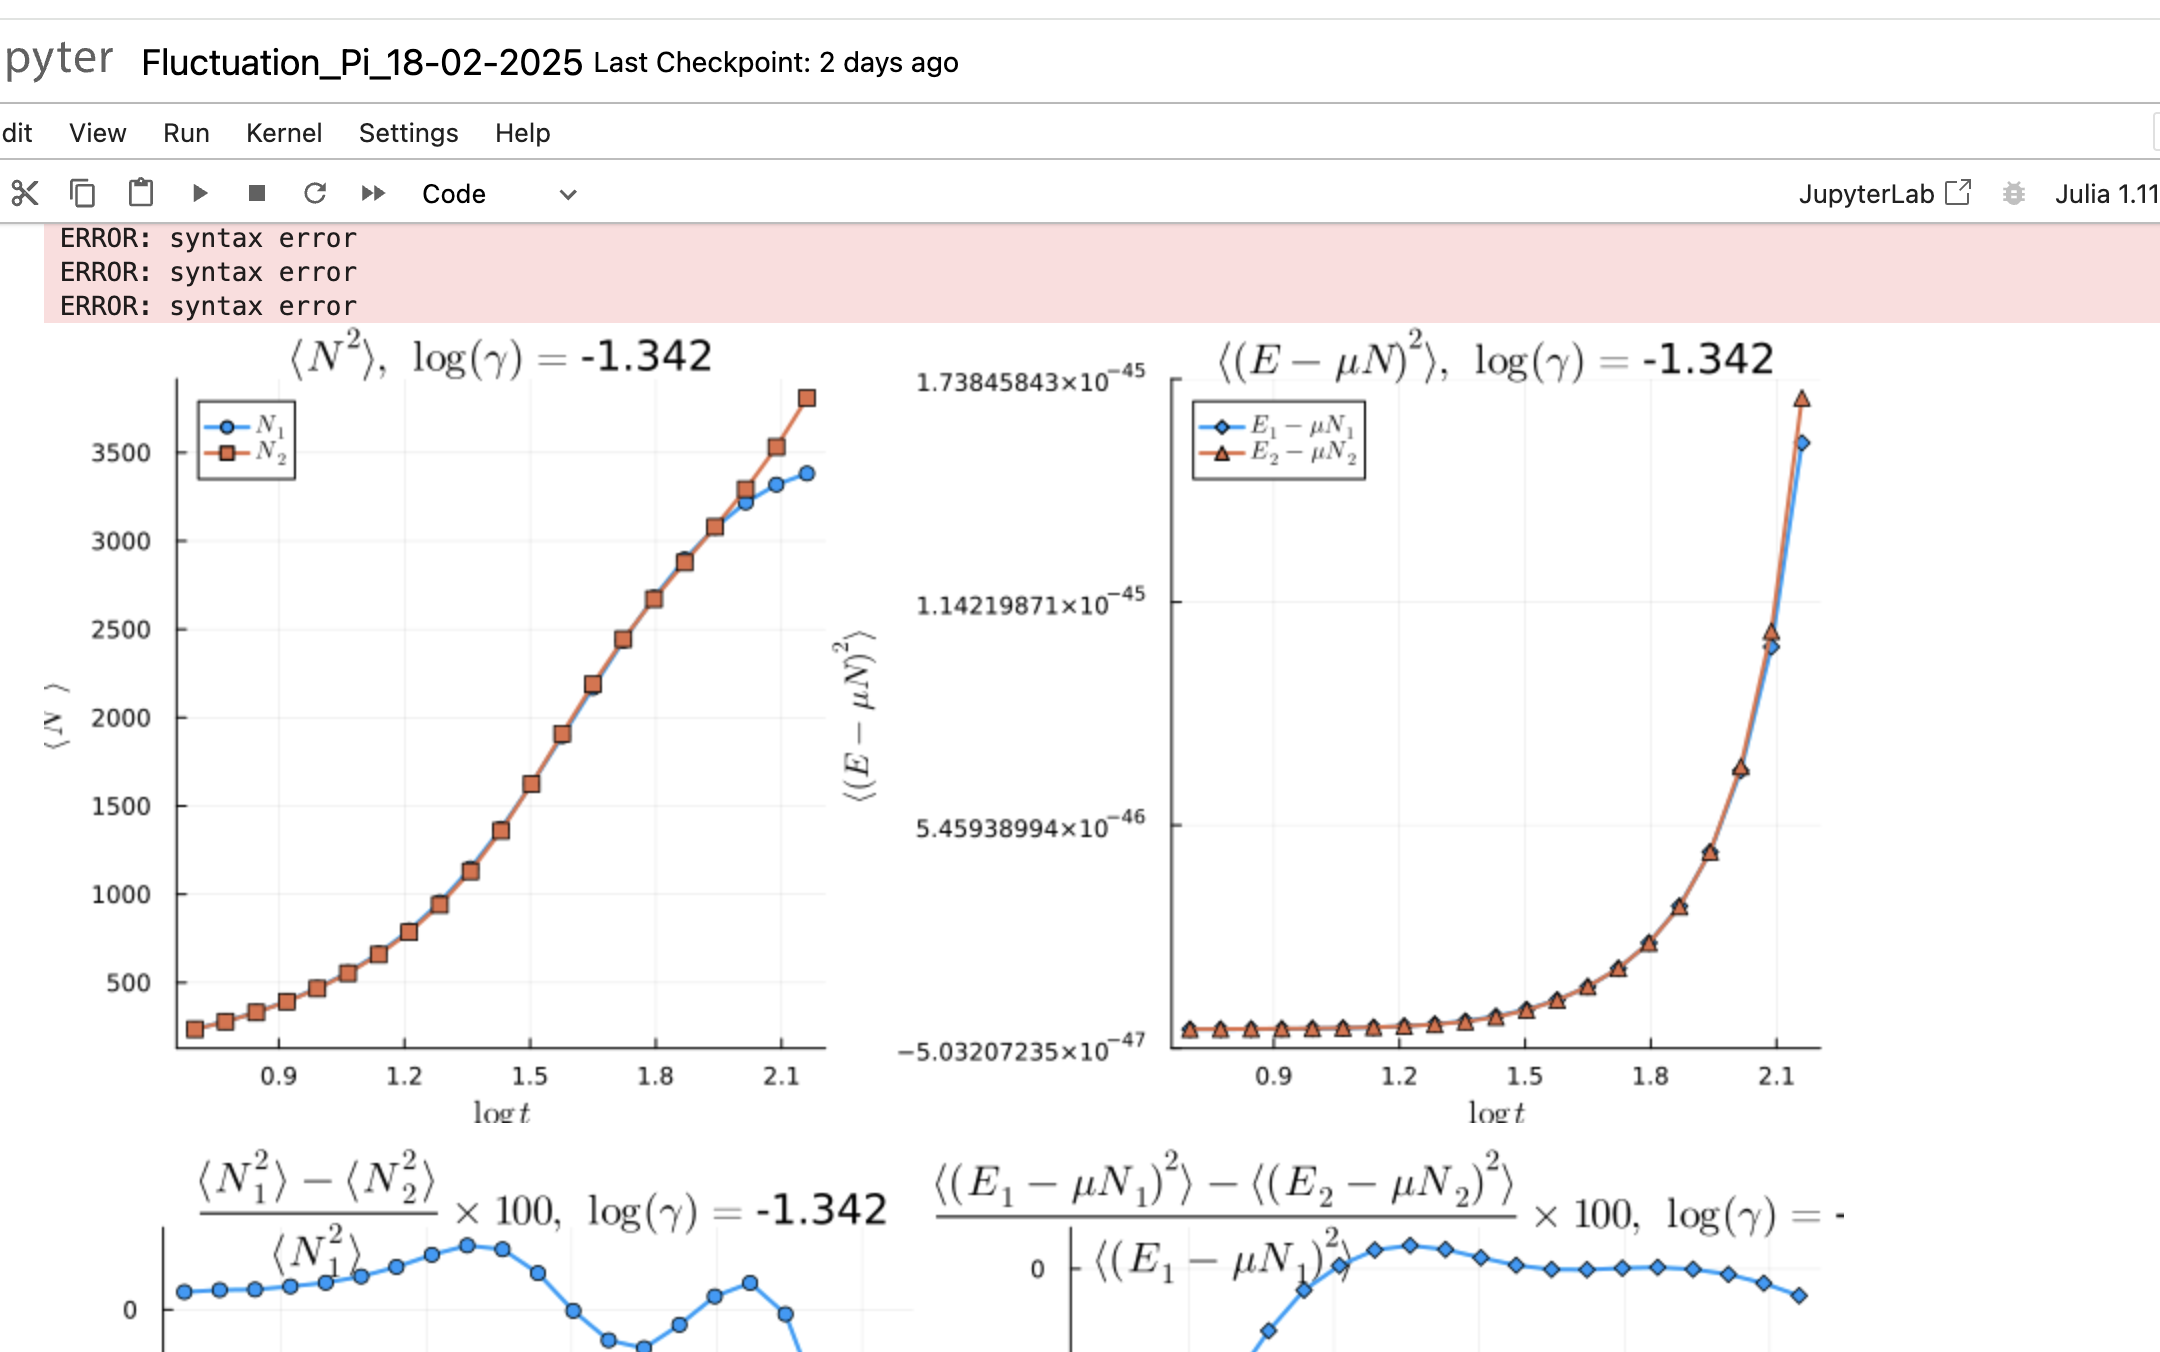
\includegraphics[width=1\textwidth]{Figures/test}

%\begin{aff}
%Donc une a l'ordre un en $\delta \theta (\operator{A}^{(0)})^{-1} %\operator{V}$ 

%\begin{eqnarray*}
%	\langle \delta \Pi ( \theta) \delta \Pi ( \theta') \rangle & = &  ( (\Pi^c_s - \Pi^c)\Pi^c/\Pi^c_s ) ( \theta ) \delta_{\theta, \theta'}/\delta \theta + \mathscr{F}(\theta , \theta' ) ,	
%\end{eqnarray*}

%avec 

%\begin{eqnarray*}
%	\mathscr{F}(\theta , \theta' ) & = & \left [ (\Pi^c_s - \Pi^c )( \theta)  +  (\Pi^c_s - \Pi^c ) ( \theta' )\right ] \frac{\Pi^c}{\Pi^c_s}(\theta)\frac{\Pi^c}{\Pi^c_s}(\theta') \frac{ \Delta( \theta'- \theta )}{ 2 \pi }\\
%	&&  - \left [ (\Pi^c_s - \Pi^c )( \theta)   (\Pi^c_s - \Pi^c ) ( \theta' )\right ] \frac{\Pi^c}{\Pi^c_s}(\theta)\frac{\Pi^c}{\Pi^c_s}(\theta')\int d\theta'' \left (   \frac{ \Pi^c/\Pi^c_s}{\Pi^c_s - \Pi^c} \right )(\theta'') \frac{\Delta(\theta''- \theta)}{2 \pi}\frac{\Delta(\theta''- \theta')}{2 \pi}  	
%\end{eqnarray*}
%\end{aff}



 









\section{Thermodynamique de Bethe et relaxation}
\subsection{Statistique des macro-états : entropie de Yang-Yang et moyennes dans le GGE}
%Dans ce chapitre, nous nous intéressons aux fluctuations de la distribution de rapidité \( \delta \rho \) autour d'une distribution de référence \( \rho^c \), qui maximise la contribution à la fonction de partition des états, exprimée comme une fonctionnelle de la distribution \( \rho \) : 

La fonction de partition des états, s'exprime comme une fonctionnelle de la distribution \( \rho \) : 

\begin{eqnarray*}
	\Xi & = & \sum_\rho \exp \left( -\mathcal{A}(\rho) \right).
\end{eqnarray*}  

Dans la section {\em \bf Entropie de Yang-Yang} (\ref{??}), l'action \( \mathcal{A}(\rho) \) s'écrit sous la forme :  

\begin{eqnarray*}
	\mathcal{A}(\rho) & \doteq & - L\mathcal{S}_{YY}(\rho) + L\int f(\theta) \rho (\theta) \, d\theta,		
\end{eqnarray*}  

où \( \mathcal{S}_{YY} \) est la fonctionnelle d'entropie de Yang-Yang, définie dans (\ref{??}), et \( f \) est la fonction paramétrant les charges, introduite dans (\ref{??}).  

Dans cette même section {\em \bf Entropie de Yang-Yang} (\ref{??}), nous avons établi un lien entre \( f \) et distribution de référence \( \rho^c \), qui maximise la contribution à la fonction de partition des états .\\

On veux tester si nos experience est décrit pas un GGE. Pour cela nous nous intéressons aux fluctuations de la distribution de rapidité \( \delta \rho \) autour \( \rho^c \).

%Nous poursuivons à présent avec cette définition de l'action de classe $\mathcal{C}^2$ et admetant une distribution critique $\rho^c$ tel que sa différentielle en ce point critique soit nulle $d\mathcal{A}_{\rho^c} = 0 $ (\ref{??}) de sorte que d'aprés la formule de Taylor-Youg %afin de déterminer les fluctuations autour de \( \Pi^c \). Pour cela, nous réécrivons l'action sous la forme :  

Nous poursuivons à présent avec cette définition de l'action de classe $\mathcal{C}^2$ et admetant une distribution critique $\rho^c$ tel que sa différentielle en ce point critique soit nulle $d\mathcal{A}_{\rho^c} = 0 $ (\ref{??}) de sorte que d'aprés la formule de Taylor-Youg %afin de déterminer les fluctuations autour de \( \Pi^c \). Pour cela, nous réécrivons l'action sous la forme :  

\begin{eqnarray*}  
	\mathcal{A}(\rho^c + \delta \rho) & \underset{ \delta \rho \to 0 }{=} & \mathcal{A}(\rho^c)  + \frac{1}{2} \left. \frac{\delta^2 \mathcal{A}}{\delta \rho^2} \right|_{\rho^c} (\delta \rho) + \mathcal{O}((\delta \rho)^3),  
\end{eqnarray*}  

une expression quadratique pour l'action à l'ordre dominant en \( \delta \Pi \) avec $\left. \frac{\delta^2 \mathcal{A}}{\delta \rho^2} \right|_{\rho^c}$ la forme quadratique définie positive (Fig (\ref{fig.fluctu.A})).

\begin{figure}[H]
	\centering 
	\begin{tikzpicture}
		\begin{scope}[shift={(0,0)}]
			\begin{scope}[transform canvas={scale=0.6}]
				% Définition des couleurs avec les codes HTML
\definecolor{colorOne}{HTML}{443E46}
\definecolor{colorTwo}{HTML}{F6DEB8}
\definecolor{colorThree}{HTML}{908CA4}
\definecolor{colorFour}{HTML}{57659E}
\definecolor{colorFive}{HTML}{C57284}
\definecolor{colorSix}{HTML}{FF5B69}

% Raccourcis pour les couleurs
\def\colorOne{colorOne}
\def\colorTwo{colorTwo}
\def\colorThree{colorThree}
\def\colorFour{colorFour}
\def\colorFive{colorFive}
\def\colorSix{colorSix}

\def\colorslide{blue!50!black}



\begin{scope}
	% Tracer une courbe lisse entre des points
	\draw[shift={(0,0)} ,\colorOne]
		(-1 , 0 ) edge [thick,line width=0.8ex , ->,>=triangle 45  , \colorOne] node [pos = 1 , below ]{\huge$\rho$}( 5  , 0 )
	;
	\draw[shift={(0,0)}, color=\colorOne]
		(0, -1.0 ) edge [thick,line width=0.8ex , ->,>=triangle 45  ]node [pos=0.9,left=0.2cm ]{\huge$\mathcal{A}(\rho)$}( 0  , 5 )
	;
	\draw[]
		(2.5, 0.12 ) edge [thick,line width=0.8ex ,\colorThree ]node [pos=1,below  ]{\huge$\rho^c$} (2.5, -0.12 )	
	;
	
	\draw[]
		(2.5, -0.12 ) edge [thick,line width=0.4ex , dashed, \colorThree ] (2.5, 5.5 )
		(1.5, 1 ) edge [thick,line width=0.4ex , <->,>=triangle 45  , \colorThree ] (3.5, 1 )
		(-0.3,1) edge [thick,line width=0.4ex  , \colorThree ] node [pos=0,left ]{\huge$\mathcal{A}(\rho^c)$} (0.3, 1 )	
	;
    \draw[thick, line width=0.8ex , \colorFour] plot[smooth, tension=0.7] coordinates {
        (1, 5) (1.6 , 3 ) (2.5, 1) (3.5 , 3 )  (4, 5)
    };		
	
\end{scope}

	
			
			\end{scope}
			
			\draw[color = red , scale = 0.5 , draw = none  ] (-2 , -1) rectangle (5, 6) ; 	
		\end{scope}
		
		\begin{scope}[shift={(19,-1)}]
			\begin{scope}[transform canvas={scale=0.6}]
				% Définition des couleurs avec les codes HTML
\definecolor{colorOne}{HTML}{443E46}
\definecolor{colorTwo}{HTML}{F6DEB8}
\definecolor{colorThree}{HTML}{908CA4}
\definecolor{colorFour}{HTML}{57659E}
\definecolor{colorFive}{HTML}{C57284}
\definecolor{colorSix}{HTML}{FF5B69}

% Raccourcis pour les couleurs
\def\colorOne{colorOne}
\def\colorTwo{colorTwo}
\def\colorThree{colorThree}
\def\colorFour{colorFour}
\def\colorFive{colorFive}
\def\colorSix{colorSix}

\def\colorslide{blue!50!black}

\def\Occupation{
	\def\traitx{0.3}
	\def\traity{0.5}
	\draw[shift={(0,0)}]
		(-13.5 , 0 ) edge [thick,line width=0.8ex ]( -3.2  , 0 )
		( -3.2 - \traitx  , 0 - \traity ) edge [thick,line width=0.8ex ]( -3.2 + \traitx  , 0 + \traity  )
		( -2.8 - \traitx  , 0 - \traity ) edge [thick,line width=0.8ex ]( -2.8 + \traitx  , 0 + \traity  )
		(-2.8 , 0 ) edge [thick,line width=0.8ex ](2.8  , 0 )
		( 2.8 - \traitx  , 0 - \traity ) edge [thick,line width=0.8ex ]( 2.8 + \traitx  , 0 + \traity  )
		( 3.2 - \traitx  , 0 - \traity ) edge [thick,line width=0.8ex ]( 3.2 + \traitx  , 0 + \traity  )
		(3.2, 0 ) edge [thick,line width=0.8ex,->,>=triangle 45 , color = black ]node [pos=1.01,below  ]{\huge$\theta$}	( 13  , 0 )
	;
	\draw[shift={(0,0)}, color=\colorOne]
		(-10.5 , -1.5 ) edge [thick,line width=0.8ex , ->,>=triangle 45  ]( -10.5  , 4.5 )
	;
		
	\foreach \r in {1 , ... , 3 } {
%		\draw[
%		decoration={
%		markings,
%    	mark connection node=my node,
%    	mark=at position 0 with{\node [blue,transform shape] (my node) {\large \r};}},
%		color=gray, thick, 
%		line width=0.5ex] decorate { 
%            (-11.0, \r) -- (-10.1, \r )}
%        ;
        \draw[
			color=\colorOne,
			] 
            (-11.0, \r) edge[color=\colorThree , thick,line width=0.5ex] node [pos=-0.5 ]{\large\color{\colorFour} $\frac{\r}{\delta \theta}$ } (-10.3, \r )
        	;
	
	}
	

	
	% Graduation abcsisse 
	% Définitions des listes
% Definitions of the lists
\def\listetuple{-9/\theta_{1}, -8/\theta_{2} , -5/\theta_{3} , -2/\theta_{a-1} , 0/\theta_{a} , 1/\theta_{a+1} , 2/\theta_{a+2} ,  5/\theta_{N-4} , 7/\theta_{N-3},8/\theta_{N-1},9/\theta_{N} }
\def\listetrais{-12 , -11, -10, -9 , -8 , -7 ,  -6 , -5, -4.5,-4, -2 , -1, 0 , 0.5, 1, 2, 4 , 5 ,  6 , 7 , 8 ,8.5, 9 ,  10 , 11, 12 }

% Loop over listetrais
\foreach \r in \listetrais {
    % Initialize found variable to zero
    % Initialize found variable to zero
    %\pgfmathsetmacro\found{0}
    \global\def\found{0}
    \xdef\nomtheta{}
    
    % Check if \r is in listetuple
    \foreach \x/\y in \listetuple { 
        \ifdim \r pt=\x pt % If \r matches any \x in listetuple
            \global\def\found{1} ;
            \xdef\nomtheta{\y} % Set \nomtheta to the corresponding \y
            %\pgfmathsetmacro\found{1} % Set found to 1            
            %\global\pgfmathsetmacro\found{1}
        \fi
    }
    
    %\node [circle, draw, red] (A) at (\r, 2) {\found , $\nomtheta$};
    
    % Draw the line and display \nomtheta if found
    \ifnum\found=1
        \draw[color=\colorOne, thick, line width=0.5ex] 
            (\r, -0.3) -- (\r, 0.3) node[red , pos=-0.5] {\large $\nomtheta$};
         \filldraw[line width=0.5ex, color=\colorSix, outer color=\colorSix, inner color=\colorSix] 
            (\r, 0) circle (4pt);
    \else 
        % Draw without \nomtheta and add a blue circle if not found
        \draw[color=\colorOne, thick, line width=0.5ex] 
            (\r, -0.3) -- (\r, 0.3);
        \filldraw[line width=0.5ex, color=\colorSix, outer color=\colorTwo, inner color=\colorTwo] 
            (\r, 0) circle (4pt); 
    \fi
}

\def\listetrais{-9.5/\theta_{i-1}/2/3, -6.5/\theta_{i}/1/4  ,   -1.5/\theta_{j}/2/4 , 1.5/\theta_{j+1}/-1/3 , 3.5/\theta_{\ell-1}/1/3 , 6.5/\theta_{\ell}/3/4 , 9.5/\theta(\theta_{\ell+1})/-1/3 };



\foreach \r/\nomx/\y/\ys in \listetrais {
	\draw[
		decoration={
		markings,
    	mark connection node=my node,
    	mark=at position .5 with{\node [blue,transform shape] (my node) {\large \color{\colorFour} $\nomx$};}},
		color=\colorThree , thick, 
		line width=0.5ex] decorate { 
            (\r, 0.12) -- (\r, -1.2)}
        ;
     
     \ifdim \y pt > -1 pt 
     	\draw[
			decoration={
			markings,
    		mark connection node=my node,
    		mark=at position .5 with{\node [blue,transform shape] (my node) {\large \color{\colorFour} $\Pi(\nomx) $};}},
			color=\colorThree, thick, 
			line width=0.5ex] decorate { 
            (\r, \y) -- (\r +3, \y)}
        ;
        \draw[
			decoration={
			markings,
    		mark connection node=my node,
    		mark=at position .5 with{\node [blue,transform shape] (my node) {\large \color{\colorFive} $\Pi_s(\nomx) $};}},
			color=\colorFive, thick, 
			line width=0.5ex] decorate { 
            (\r, \ys) -- (\r +3, \ys)}
        ;
     \fi 
     \ifdim \r pt= -1.5 pt
     	\draw[
     		decoration={
			markings,
    		mark connection node=my node,
    		mark=at position .5 with{\node [blue,transform shape] (my node) {\large \color{\colorFour}  $\delta \theta $};},
    		%mark=at position 0.1  with {\arrow[blue, line width=0.5ex]{<}},
    		%mark=at position 1  with {\arrow[blue, line width=0.5ex]{>}}
    		},
        	color=\colorThree,
        	thick,
        	line width=0.5ex,
        	%arrows={Computer Modern Rightarrow[line cap=round]-Computer Modern Rightarrow[line cap=round]}
   			](\r, -1.2) edge[arrows={Computer Modern Rightarrow[line cap=round]-}] (\r + 0.4, -1.2)decorate {
    		(\r, -1.2) -- (\r + 3, -1.2)}(\r + 2, -1.2) edge[arrows={-Computer Modern Rightarrow[line cap=round]}] (\r + 3, -1.2)
    		;
    \fi
			
	
}


			
}


\begin{scope}
	%\draw[help lines , width=1.5ex] (-8,-3) grid (8,3);\draw[help lines ,width=0.5ex , opacity = 0.5] (-3,-3) grid[step=0.1] (3,3));
	
	%\draw[help lines] 
	%	(-3,-3) edge[width=1.5ex] grid (3,3)	
	%	(-3,-3) edge[width=0.5ex , opacity = 0.5] grid (3,3)	
	%;
	\begin{scope}[shift={(0,1)},rotate=0,opacity=1,color=black]
		\Occupation	
		
		%\node[anchor=east, font=\bfseries] at (-11, 0) {\color{red}\large (T = 0 )} ;	
	\end{scope}
	
	
	
	
	\begin{scope}[shift={(-10.5,7)},rotate=0,opacity=1,color=black]
	
	\begin{scope}[shift={(-0,0)},rotate=0,opacity=1,color=black]
	
		\draw[shift={(0,0)} ,line width=1ex,rounded corners = 1ex,color=\colorOne , opacity =1 ,fill=\colorOne!00 , pattern={north east lines} , pattern color=\colorOne!00 ]
			(0 , -1 ) rectangle (5,1)
		;
		

		\begin{scope}[shift={(0.5,0.5)}]
			\draw[color=\colorOne, thick, line width=0.5ex] 
            (0, -0.3) -- (0, 0.3) ;
            \filldraw[line width=0.5ex, color=\colorSix, outer color=\colorSix, inner color=\colorSix] 
            (0, 0) circle (4pt);
            
            \node[anchor=west, font=\bfseries] at (0.2, 0) {\color{\colorSix}\large : quasi-particule};
		\end{scope}
		
		\begin{scope}[shift={(0.5,-0.5)}]
			\draw[color=\colorOne, thick, line width=0.5ex] 
            (0, -0.3) -- (0, 0.3) ;
            \filldraw[line width=0.5ex, color=\colorSix, outer color=\colorTwo, inner color=\colorTwo] 
            (0, 0) circle (4pt);
            
            \node[anchor=west, font=\bfseries] at (0.2, 0) {\color{\colorSix}\large : hole};
		\end{scope}

	\end{scope}
	
	\begin{scope}[shift={(6,0)},rotate=0,opacity=1,color=black]	
		
		\draw[shift={(0,0)} ,line width=1ex,rounded corners = 1ex,color=\colorOne , opacity =1 ,fill=\colorOne!00 , pattern={north east lines} , pattern color=\colorOne!00 ]
			(0 , -1 ) rectangle (7.5,1)
		;
		
		\node[anchor=west] at (0.5, 0.5) {\color{\colorFour}\large $\Pi$ };\node[anchor=west, font=\bfseries] at (1, 0.5) {\color{\colorFour}\large : quasi-particule distribution};
		
		\node[anchor=west] at (0.5, -0.5) {\color{\colorFour}\large $\Pi_h$ };\node[anchor=west, font=\bfseries] at (1, -0.5) {\color{\colorFour}\large  : hole distribution};
		
	\end{scope}
	
	\begin{scope}[shift={(14.5,0)},rotate=0,opacity=1,color=black]	
		
		\draw[shift={(0,0)} ,line width=1ex,rounded corners = 1ex,color=\colorOne , opacity =1 ,fill=\colorOne!00 , pattern={north east lines} , pattern color=\colorOne!00 ]
			(0 , -0.5 ) rectangle (7.0,0.5)
		;
		
		\node[anchor=west] at (0.2, 0) {\color{\colorFour}\large ${\color{\colorFive}\Pi_s} = \Pi + \Pi_h $ } node[anchor=west , font=\bfseries] at (3.1 , 0 )  {\color{\colorFour}\large {\color{\colorFive} : density of states}};
		
	\end{scope}
	
	
	\end{scope}


		
	
\end{scope}

	
			
			\end{scope}
			\begin{scope}[scale=1]
				\draw[color = red , scale = 1 , draw = none  ] (-1 , -1) rectangle (5, 5) ; 
			\end{scope}	
		\end{scope}

		
				
			
	\end{tikzpicture}	
	\captionsetup{skip=10pt} % Ajoute de l’espace après la légende
	\label{fig.fluctu.A}
\end{figure}


On discrétise l'axe des rapidités en  petite cellule de rapidité $[\theta, \theta+\delta\theta]$, qui contient $L\rho(\theta) \delta \theta$ rapidités. 
	



Avec ces petites tranches, la forme quadratique s’écrit :

\begin{eqnarray*}
    \left. \frac{\delta^2 \mathcal{A}}{{\delta \rho}^2} \right|_{\rho^c}(\delta \rho ) &=&  \sum_{a,b \mid \text{tranche}}  
    \delta \rho(\theta_a)  \frac{\partial^2 \mathcal{A}}{\partial \delta \rho(\theta_a) \partial \delta \rho(\theta_b) } (\rho^c)  \delta \rho(\theta_b).
\end{eqnarray*}
Les fluctuations s’écrivent donc :

\begin{eqnarray*}
    \langle \delta \rho ( \theta) \delta \rho ( \theta') \rangle &=&  
    \frac{ \int d\delta \rho \, \delta \rho(\theta) \delta \rho ( \theta') 
    \exp \left( - \frac{1}{2} \sum_{a,b \mid \text{tranche}}  
    \delta \rho(\theta_a) \frac{\partial^2 \mathcal{A}}{\partial \delta \rho(\theta_a) \partial \delta \rho(\theta_b) } (\rho^c)  \delta \rho(\theta_b) \right) }
    { \int d\delta \Pi  
    \exp \left( - \frac{1}{2} \sum_{a,b \mid \text{tranche}}  
    \delta \rho(\theta_a) \frac{\partial^2 \mathcal{A}}{\partial \delta \rho(\theta_a) \partial \delta \rho(\theta_b) } (\rho^c)  \delta \rho(\theta_b) \right) } \\
    &=& \left( \mathbf{A}^{-1} \right)_{\theta , \theta'}
\end{eqnarray*}


\begin{aff}

\begin{eqnarray*}
	\langle \delta \rho ( \theta) \delta \rho ( \theta') \rangle &=& 	\left( \mathbf{A}^{-1} \right)_{\theta , \theta'}
\end{eqnarray*}

	
avec la  {\em matrice hessienne} $\mathbf{A}_{\theta , \theta'} \equiv \frac{\partial^2 \mathcal{A}}{\partial \delta \rho(\theta) \partial \delta \rho(\theta') }(\rho^c)$, au point critique/ qui maximise la probabilité  $\rho^c=\rho^c_s \nu^c $, s'écrit

\begin{eqnarray*}
	\operator{A} & = & \operator{A}^{(0)} + \delta \theta \operator{V}
\end{eqnarray*}

avec 

\begin{eqnarray*}
	A^{(0)}_{\theta , \theta'}  & = &  L\delta \theta \left ( \frac{ 1}{\rho^c_s ( 1  - \nu^c ) \nu^c } \right )(\theta)    \delta({\theta - \theta '})	,\\
	V_{\theta , \theta'}  &= & L \delta \theta \left \{ - \left [ \left ( \frac{1}{\rho^c_s( 1 - \nu^c) } \right ) ( \theta)  +  \left ( \frac{1}{\rho^c_s( 1 - \nu^c) } \right ) ( \theta' )\right ] \frac{ \Delta( \theta'- \theta )}{ 2 \pi } + \int d\theta''  \left ( \frac{\nu^c}{\rho^c_s( 1 - \nu^c) } \right )(\theta'') \frac{\Delta(\theta''- \theta)}{2 \pi}\frac{\Delta(\theta''- \theta')}{2 \pi}   \right \} 	
\end{eqnarray*}

\end{aff}

\subsection{Testes}

\begin{eqnarray*}
	\Delta_{\operator{\mathcal{N}}}^2  & = &  \frac{1}{\beta} \left . \frac{\partial \langle \operator{\mathcal{N}} \rangle}{\partial \mu} \right )_T \\
	\Delta_{\operator{\mathcal{E}}-\mu \operator{\mathcal{N}}}^2  & = &  - \left . \frac{\partial \langle \operator{\mathcal{E}}-\mu \operator{\mathcal{N}} \rangle}{\partial \beta} \right )_\mu 
\end{eqnarray*}

et 

\begin{eqnarray*}
	\Delta_{\operator{\mathcal{N}}}^2  &= & L^2 \int d\theta_a \int d \theta_b \, \langle \delta \rho(\theta_a) \delta \rho(\theta_b) \rangle \\
	\Delta_{\operator{\mathcal{E}}-\mu \operator{\mathcal{N}}}^2  & = & L^2 \int d\theta_a \int d \theta_b \, \left ( - \mu + \frac{1}2 m \theta_a^2  \right  )\left ( - \mu + \frac{1}2 m \theta_b^2  \right  )  \langle \delta \rho(\theta_a) \delta \rho(\theta_b) \rangle
\end{eqnarray*}

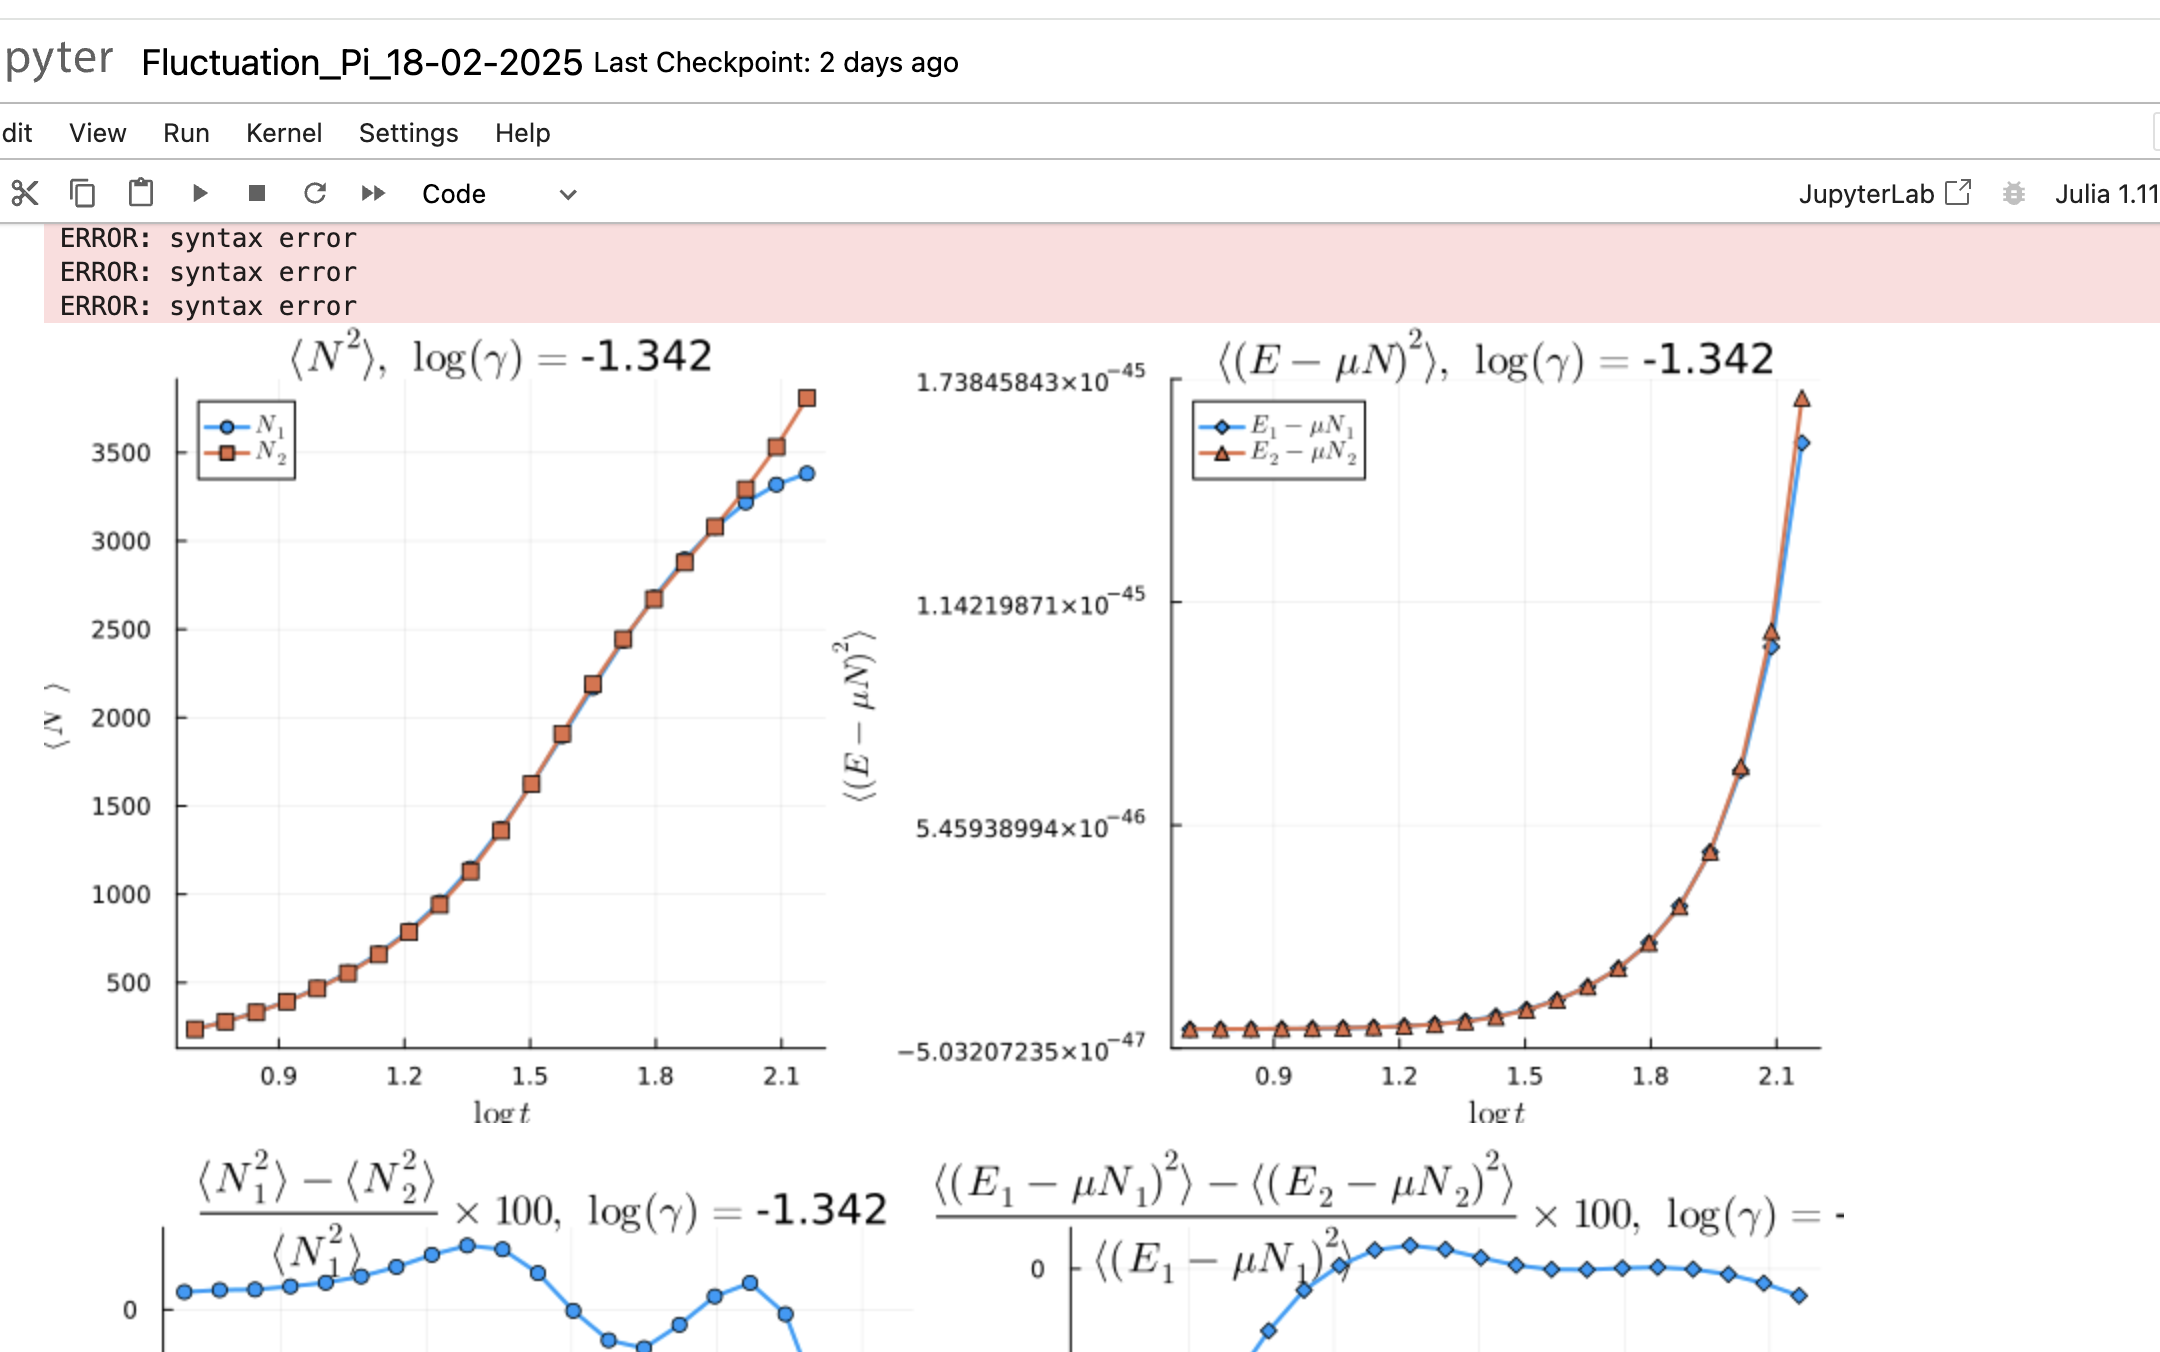
\includegraphics[width=1\textwidth]{Figures/test}

%\begin{aff}
%Donc une a l'ordre un en $\delta \theta (\operator{A}^{(0)})^{-1} %\operator{V}$ 

%\begin{eqnarray*}
%	\langle \delta \Pi ( \theta) \delta \Pi ( \theta') \rangle & = &  ( (\Pi^c_s - \Pi^c)\Pi^c/\Pi^c_s ) ( \theta ) \delta_{\theta, \theta'}/\delta \theta + \mathscr{F}(\theta , \theta' ) ,	
%\end{eqnarray*}

%avec 

%\begin{eqnarray*}
%	\mathscr{F}(\theta , \theta' ) & = & \left [ (\Pi^c_s - \Pi^c )( \theta)  +  (\Pi^c_s - \Pi^c ) ( \theta' )\right ] \frac{\Pi^c}{\Pi^c_s}(\theta)\frac{\Pi^c}{\Pi^c_s}(\theta') \frac{ \Delta( \theta'- \theta )}{ 2 \pi }\\
%	&&  - \left [ (\Pi^c_s - \Pi^c )( \theta)   (\Pi^c_s - \Pi^c ) ( \theta' )\right ] \frac{\Pi^c}{\Pi^c_s}(\theta)\frac{\Pi^c}{\Pi^c_s}(\theta')\int d\theta'' \left (   \frac{ \Pi^c/\Pi^c_s}{\Pi^c_s - \Pi^c} \right )(\theta'') \frac{\Delta(\theta''- \theta)}{2 \pi}\frac{\Delta(\theta''- \theta')}{2 \pi}  	
%\end{eqnarray*}
%\end{aff}



 








\subsection{Équations intégrales de la TBA}
%Dans ce chapitre, nous nous intéressons aux fluctuations de la distribution de rapidité \( \delta \rho \) autour d'une distribution de référence \( \rho^c \), qui maximise la contribution à la fonction de partition des états, exprimée comme une fonctionnelle de la distribution \( \rho \) : 

La fonction de partition des états, s'exprime comme une fonctionnelle de la distribution \( \rho \) : 

\begin{eqnarray*}
	\Xi & = & \sum_\rho \exp \left( -\mathcal{A}(\rho) \right).
\end{eqnarray*}  

Dans la section {\em \bf Entropie de Yang-Yang} (\ref{??}), l'action \( \mathcal{A}(\rho) \) s'écrit sous la forme :  

\begin{eqnarray*}
	\mathcal{A}(\rho) & \doteq & - L\mathcal{S}_{YY}(\rho) + L\int f(\theta) \rho (\theta) \, d\theta,		
\end{eqnarray*}  

où \( \mathcal{S}_{YY} \) est la fonctionnelle d'entropie de Yang-Yang, définie dans (\ref{??}), et \( f \) est la fonction paramétrant les charges, introduite dans (\ref{??}).  

Dans cette même section {\em \bf Entropie de Yang-Yang} (\ref{??}), nous avons établi un lien entre \( f \) et distribution de référence \( \rho^c \), qui maximise la contribution à la fonction de partition des états .\\

On veux tester si nos experience est décrit pas un GGE. Pour cela nous nous intéressons aux fluctuations de la distribution de rapidité \( \delta \rho \) autour \( \rho^c \).

%Nous poursuivons à présent avec cette définition de l'action de classe $\mathcal{C}^2$ et admetant une distribution critique $\rho^c$ tel que sa différentielle en ce point critique soit nulle $d\mathcal{A}_{\rho^c} = 0 $ (\ref{??}) de sorte que d'aprés la formule de Taylor-Youg %afin de déterminer les fluctuations autour de \( \Pi^c \). Pour cela, nous réécrivons l'action sous la forme :  

Nous poursuivons à présent avec cette définition de l'action de classe $\mathcal{C}^2$ et admetant une distribution critique $\rho^c$ tel que sa différentielle en ce point critique soit nulle $d\mathcal{A}_{\rho^c} = 0 $ (\ref{??}) de sorte que d'aprés la formule de Taylor-Youg %afin de déterminer les fluctuations autour de \( \Pi^c \). Pour cela, nous réécrivons l'action sous la forme :  

\begin{eqnarray*}  
	\mathcal{A}(\rho^c + \delta \rho) & \underset{ \delta \rho \to 0 }{=} & \mathcal{A}(\rho^c)  + \frac{1}{2} \left. \frac{\delta^2 \mathcal{A}}{\delta \rho^2} \right|_{\rho^c} (\delta \rho) + \mathcal{O}((\delta \rho)^3),  
\end{eqnarray*}  

une expression quadratique pour l'action à l'ordre dominant en \( \delta \Pi \) avec $\left. \frac{\delta^2 \mathcal{A}}{\delta \rho^2} \right|_{\rho^c}$ la forme quadratique définie positive (Fig (\ref{fig.fluctu.A})).

\begin{figure}[H]
	\centering 
	\begin{tikzpicture}
		\begin{scope}[shift={(0,0)}]
			\begin{scope}[transform canvas={scale=0.6}]
				% Définition des couleurs avec les codes HTML
\definecolor{colorOne}{HTML}{443E46}
\definecolor{colorTwo}{HTML}{F6DEB8}
\definecolor{colorThree}{HTML}{908CA4}
\definecolor{colorFour}{HTML}{57659E}
\definecolor{colorFive}{HTML}{C57284}
\definecolor{colorSix}{HTML}{FF5B69}

% Raccourcis pour les couleurs
\def\colorOne{colorOne}
\def\colorTwo{colorTwo}
\def\colorThree{colorThree}
\def\colorFour{colorFour}
\def\colorFive{colorFive}
\def\colorSix{colorSix}

\def\colorslide{blue!50!black}



\begin{scope}
	% Tracer une courbe lisse entre des points
	\draw[shift={(0,0)} ,\colorOne]
		(-1 , 0 ) edge [thick,line width=0.8ex , ->,>=triangle 45  , \colorOne] node [pos = 1 , below ]{\huge$\rho$}( 5  , 0 )
	;
	\draw[shift={(0,0)}, color=\colorOne]
		(0, -1.0 ) edge [thick,line width=0.8ex , ->,>=triangle 45  ]node [pos=0.9,left=0.2cm ]{\huge$\mathcal{A}(\rho)$}( 0  , 5 )
	;
	\draw[]
		(2.5, 0.12 ) edge [thick,line width=0.8ex ,\colorThree ]node [pos=1,below  ]{\huge$\rho^c$} (2.5, -0.12 )	
	;
	
	\draw[]
		(2.5, -0.12 ) edge [thick,line width=0.4ex , dashed, \colorThree ] (2.5, 5.5 )
		(1.5, 1 ) edge [thick,line width=0.4ex , <->,>=triangle 45  , \colorThree ] (3.5, 1 )
		(-0.3,1) edge [thick,line width=0.4ex  , \colorThree ] node [pos=0,left ]{\huge$\mathcal{A}(\rho^c)$} (0.3, 1 )	
	;
    \draw[thick, line width=0.8ex , \colorFour] plot[smooth, tension=0.7] coordinates {
        (1, 5) (1.6 , 3 ) (2.5, 1) (3.5 , 3 )  (4, 5)
    };		
	
\end{scope}

	
			
			\end{scope}
			
			\draw[color = red , scale = 0.5 , draw = none  ] (-2 , -1) rectangle (5, 6) ; 	
		\end{scope}
		
		\begin{scope}[shift={(19,-1)}]
			\begin{scope}[transform canvas={scale=0.6}]
				% Définition des couleurs avec les codes HTML
\definecolor{colorOne}{HTML}{443E46}
\definecolor{colorTwo}{HTML}{F6DEB8}
\definecolor{colorThree}{HTML}{908CA4}
\definecolor{colorFour}{HTML}{57659E}
\definecolor{colorFive}{HTML}{C57284}
\definecolor{colorSix}{HTML}{FF5B69}

% Raccourcis pour les couleurs
\def\colorOne{colorOne}
\def\colorTwo{colorTwo}
\def\colorThree{colorThree}
\def\colorFour{colorFour}
\def\colorFive{colorFive}
\def\colorSix{colorSix}

\def\colorslide{blue!50!black}

\def\Occupation{
	\def\traitx{0.3}
	\def\traity{0.5}
	\draw[shift={(0,0)}]
		(-13.5 , 0 ) edge [thick,line width=0.8ex ]( -3.2  , 0 )
		( -3.2 - \traitx  , 0 - \traity ) edge [thick,line width=0.8ex ]( -3.2 + \traitx  , 0 + \traity  )
		( -2.8 - \traitx  , 0 - \traity ) edge [thick,line width=0.8ex ]( -2.8 + \traitx  , 0 + \traity  )
		(-2.8 , 0 ) edge [thick,line width=0.8ex ](2.8  , 0 )
		( 2.8 - \traitx  , 0 - \traity ) edge [thick,line width=0.8ex ]( 2.8 + \traitx  , 0 + \traity  )
		( 3.2 - \traitx  , 0 - \traity ) edge [thick,line width=0.8ex ]( 3.2 + \traitx  , 0 + \traity  )
		(3.2, 0 ) edge [thick,line width=0.8ex,->,>=triangle 45 , color = black ]node [pos=1.01,below  ]{\huge$\theta$}	( 13  , 0 )
	;
	\draw[shift={(0,0)}, color=\colorOne]
		(-10.5 , -1.5 ) edge [thick,line width=0.8ex , ->,>=triangle 45  ]( -10.5  , 4.5 )
	;
		
	\foreach \r in {1 , ... , 3 } {
%		\draw[
%		decoration={
%		markings,
%    	mark connection node=my node,
%    	mark=at position 0 with{\node [blue,transform shape] (my node) {\large \r};}},
%		color=gray, thick, 
%		line width=0.5ex] decorate { 
%            (-11.0, \r) -- (-10.1, \r )}
%        ;
        \draw[
			color=\colorOne,
			] 
            (-11.0, \r) edge[color=\colorThree , thick,line width=0.5ex] node [pos=-0.5 ]{\large\color{\colorFour} $\frac{\r}{\delta \theta}$ } (-10.3, \r )
        	;
	
	}
	

	
	% Graduation abcsisse 
	% Définitions des listes
% Definitions of the lists
\def\listetuple{-9/\theta_{1}, -8/\theta_{2} , -5/\theta_{3} , -2/\theta_{a-1} , 0/\theta_{a} , 1/\theta_{a+1} , 2/\theta_{a+2} ,  5/\theta_{N-4} , 7/\theta_{N-3},8/\theta_{N-1},9/\theta_{N} }
\def\listetrais{-12 , -11, -10, -9 , -8 , -7 ,  -6 , -5, -4.5,-4, -2 , -1, 0 , 0.5, 1, 2, 4 , 5 ,  6 , 7 , 8 ,8.5, 9 ,  10 , 11, 12 }

% Loop over listetrais
\foreach \r in \listetrais {
    % Initialize found variable to zero
    % Initialize found variable to zero
    %\pgfmathsetmacro\found{0}
    \global\def\found{0}
    \xdef\nomtheta{}
    
    % Check if \r is in listetuple
    \foreach \x/\y in \listetuple { 
        \ifdim \r pt=\x pt % If \r matches any \x in listetuple
            \global\def\found{1} ;
            \xdef\nomtheta{\y} % Set \nomtheta to the corresponding \y
            %\pgfmathsetmacro\found{1} % Set found to 1            
            %\global\pgfmathsetmacro\found{1}
        \fi
    }
    
    %\node [circle, draw, red] (A) at (\r, 2) {\found , $\nomtheta$};
    
    % Draw the line and display \nomtheta if found
    \ifnum\found=1
        \draw[color=\colorOne, thick, line width=0.5ex] 
            (\r, -0.3) -- (\r, 0.3) node[red , pos=-0.5] {\large $\nomtheta$};
         \filldraw[line width=0.5ex, color=\colorSix, outer color=\colorSix, inner color=\colorSix] 
            (\r, 0) circle (4pt);
    \else 
        % Draw without \nomtheta and add a blue circle if not found
        \draw[color=\colorOne, thick, line width=0.5ex] 
            (\r, -0.3) -- (\r, 0.3);
        \filldraw[line width=0.5ex, color=\colorSix, outer color=\colorTwo, inner color=\colorTwo] 
            (\r, 0) circle (4pt); 
    \fi
}

\def\listetrais{-9.5/\theta_{i-1}/2/3, -6.5/\theta_{i}/1/4  ,   -1.5/\theta_{j}/2/4 , 1.5/\theta_{j+1}/-1/3 , 3.5/\theta_{\ell-1}/1/3 , 6.5/\theta_{\ell}/3/4 , 9.5/\theta(\theta_{\ell+1})/-1/3 };



\foreach \r/\nomx/\y/\ys in \listetrais {
	\draw[
		decoration={
		markings,
    	mark connection node=my node,
    	mark=at position .5 with{\node [blue,transform shape] (my node) {\large \color{\colorFour} $\nomx$};}},
		color=\colorThree , thick, 
		line width=0.5ex] decorate { 
            (\r, 0.12) -- (\r, -1.2)}
        ;
     
     \ifdim \y pt > -1 pt 
     	\draw[
			decoration={
			markings,
    		mark connection node=my node,
    		mark=at position .5 with{\node [blue,transform shape] (my node) {\large \color{\colorFour} $\Pi(\nomx) $};}},
			color=\colorThree, thick, 
			line width=0.5ex] decorate { 
            (\r, \y) -- (\r +3, \y)}
        ;
        \draw[
			decoration={
			markings,
    		mark connection node=my node,
    		mark=at position .5 with{\node [blue,transform shape] (my node) {\large \color{\colorFive} $\Pi_s(\nomx) $};}},
			color=\colorFive, thick, 
			line width=0.5ex] decorate { 
            (\r, \ys) -- (\r +3, \ys)}
        ;
     \fi 
     \ifdim \r pt= -1.5 pt
     	\draw[
     		decoration={
			markings,
    		mark connection node=my node,
    		mark=at position .5 with{\node [blue,transform shape] (my node) {\large \color{\colorFour}  $\delta \theta $};},
    		%mark=at position 0.1  with {\arrow[blue, line width=0.5ex]{<}},
    		%mark=at position 1  with {\arrow[blue, line width=0.5ex]{>}}
    		},
        	color=\colorThree,
        	thick,
        	line width=0.5ex,
        	%arrows={Computer Modern Rightarrow[line cap=round]-Computer Modern Rightarrow[line cap=round]}
   			](\r, -1.2) edge[arrows={Computer Modern Rightarrow[line cap=round]-}] (\r + 0.4, -1.2)decorate {
    		(\r, -1.2) -- (\r + 3, -1.2)}(\r + 2, -1.2) edge[arrows={-Computer Modern Rightarrow[line cap=round]}] (\r + 3, -1.2)
    		;
    \fi
			
	
}


			
}


\begin{scope}
	%\draw[help lines , width=1.5ex] (-8,-3) grid (8,3);\draw[help lines ,width=0.5ex , opacity = 0.5] (-3,-3) grid[step=0.1] (3,3));
	
	%\draw[help lines] 
	%	(-3,-3) edge[width=1.5ex] grid (3,3)	
	%	(-3,-3) edge[width=0.5ex , opacity = 0.5] grid (3,3)	
	%;
	\begin{scope}[shift={(0,1)},rotate=0,opacity=1,color=black]
		\Occupation	
		
		%\node[anchor=east, font=\bfseries] at (-11, 0) {\color{red}\large (T = 0 )} ;	
	\end{scope}
	
	
	
	
	\begin{scope}[shift={(-10.5,7)},rotate=0,opacity=1,color=black]
	
	\begin{scope}[shift={(-0,0)},rotate=0,opacity=1,color=black]
	
		\draw[shift={(0,0)} ,line width=1ex,rounded corners = 1ex,color=\colorOne , opacity =1 ,fill=\colorOne!00 , pattern={north east lines} , pattern color=\colorOne!00 ]
			(0 , -1 ) rectangle (5,1)
		;
		

		\begin{scope}[shift={(0.5,0.5)}]
			\draw[color=\colorOne, thick, line width=0.5ex] 
            (0, -0.3) -- (0, 0.3) ;
            \filldraw[line width=0.5ex, color=\colorSix, outer color=\colorSix, inner color=\colorSix] 
            (0, 0) circle (4pt);
            
            \node[anchor=west, font=\bfseries] at (0.2, 0) {\color{\colorSix}\large : quasi-particule};
		\end{scope}
		
		\begin{scope}[shift={(0.5,-0.5)}]
			\draw[color=\colorOne, thick, line width=0.5ex] 
            (0, -0.3) -- (0, 0.3) ;
            \filldraw[line width=0.5ex, color=\colorSix, outer color=\colorTwo, inner color=\colorTwo] 
            (0, 0) circle (4pt);
            
            \node[anchor=west, font=\bfseries] at (0.2, 0) {\color{\colorSix}\large : hole};
		\end{scope}

	\end{scope}
	
	\begin{scope}[shift={(6,0)},rotate=0,opacity=1,color=black]	
		
		\draw[shift={(0,0)} ,line width=1ex,rounded corners = 1ex,color=\colorOne , opacity =1 ,fill=\colorOne!00 , pattern={north east lines} , pattern color=\colorOne!00 ]
			(0 , -1 ) rectangle (7.5,1)
		;
		
		\node[anchor=west] at (0.5, 0.5) {\color{\colorFour}\large $\Pi$ };\node[anchor=west, font=\bfseries] at (1, 0.5) {\color{\colorFour}\large : quasi-particule distribution};
		
		\node[anchor=west] at (0.5, -0.5) {\color{\colorFour}\large $\Pi_h$ };\node[anchor=west, font=\bfseries] at (1, -0.5) {\color{\colorFour}\large  : hole distribution};
		
	\end{scope}
	
	\begin{scope}[shift={(14.5,0)},rotate=0,opacity=1,color=black]	
		
		\draw[shift={(0,0)} ,line width=1ex,rounded corners = 1ex,color=\colorOne , opacity =1 ,fill=\colorOne!00 , pattern={north east lines} , pattern color=\colorOne!00 ]
			(0 , -0.5 ) rectangle (7.0,0.5)
		;
		
		\node[anchor=west] at (0.2, 0) {\color{\colorFour}\large ${\color{\colorFive}\Pi_s} = \Pi + \Pi_h $ } node[anchor=west , font=\bfseries] at (3.1 , 0 )  {\color{\colorFour}\large {\color{\colorFive} : density of states}};
		
	\end{scope}
	
	
	\end{scope}


		
	
\end{scope}

	
			
			\end{scope}
			\begin{scope}[scale=1]
				\draw[color = red , scale = 1 , draw = none  ] (-1 , -1) rectangle (5, 5) ; 
			\end{scope}	
		\end{scope}

		
				
			
	\end{tikzpicture}	
	\captionsetup{skip=10pt} % Ajoute de l’espace après la légende
	\label{fig.fluctu.A}
\end{figure}


On discrétise l'axe des rapidités en  petite cellule de rapidité $[\theta, \theta+\delta\theta]$, qui contient $L\rho(\theta) \delta \theta$ rapidités. 
	



Avec ces petites tranches, la forme quadratique s’écrit :

\begin{eqnarray*}
    \left. \frac{\delta^2 \mathcal{A}}{{\delta \rho}^2} \right|_{\rho^c}(\delta \rho ) &=&  \sum_{a,b \mid \text{tranche}}  
    \delta \rho(\theta_a)  \frac{\partial^2 \mathcal{A}}{\partial \delta \rho(\theta_a) \partial \delta \rho(\theta_b) } (\rho^c)  \delta \rho(\theta_b).
\end{eqnarray*}
Les fluctuations s’écrivent donc :

\begin{eqnarray*}
    \langle \delta \rho ( \theta) \delta \rho ( \theta') \rangle &=&  
    \frac{ \int d\delta \rho \, \delta \rho(\theta) \delta \rho ( \theta') 
    \exp \left( - \frac{1}{2} \sum_{a,b \mid \text{tranche}}  
    \delta \rho(\theta_a) \frac{\partial^2 \mathcal{A}}{\partial \delta \rho(\theta_a) \partial \delta \rho(\theta_b) } (\rho^c)  \delta \rho(\theta_b) \right) }
    { \int d\delta \Pi  
    \exp \left( - \frac{1}{2} \sum_{a,b \mid \text{tranche}}  
    \delta \rho(\theta_a) \frac{\partial^2 \mathcal{A}}{\partial \delta \rho(\theta_a) \partial \delta \rho(\theta_b) } (\rho^c)  \delta \rho(\theta_b) \right) } \\
    &=& \left( \mathbf{A}^{-1} \right)_{\theta , \theta'}
\end{eqnarray*}


\begin{aff}

\begin{eqnarray*}
	\langle \delta \rho ( \theta) \delta \rho ( \theta') \rangle &=& 	\left( \mathbf{A}^{-1} \right)_{\theta , \theta'}
\end{eqnarray*}

	
avec la  {\em matrice hessienne} $\mathbf{A}_{\theta , \theta'} \equiv \frac{\partial^2 \mathcal{A}}{\partial \delta \rho(\theta) \partial \delta \rho(\theta') }(\rho^c)$, au point critique/ qui maximise la probabilité  $\rho^c=\rho^c_s \nu^c $, s'écrit

\begin{eqnarray*}
	\operator{A} & = & \operator{A}^{(0)} + \delta \theta \operator{V}
\end{eqnarray*}

avec 

\begin{eqnarray*}
	A^{(0)}_{\theta , \theta'}  & = &  L\delta \theta \left ( \frac{ 1}{\rho^c_s ( 1  - \nu^c ) \nu^c } \right )(\theta)    \delta({\theta - \theta '})	,\\
	V_{\theta , \theta'}  &= & L \delta \theta \left \{ - \left [ \left ( \frac{1}{\rho^c_s( 1 - \nu^c) } \right ) ( \theta)  +  \left ( \frac{1}{\rho^c_s( 1 - \nu^c) } \right ) ( \theta' )\right ] \frac{ \Delta( \theta'- \theta )}{ 2 \pi } + \int d\theta''  \left ( \frac{\nu^c}{\rho^c_s( 1 - \nu^c) } \right )(\theta'') \frac{\Delta(\theta''- \theta)}{2 \pi}\frac{\Delta(\theta''- \theta')}{2 \pi}   \right \} 	
\end{eqnarray*}

\end{aff}

\subsection{Testes}

\begin{eqnarray*}
	\Delta_{\operator{\mathcal{N}}}^2  & = &  \frac{1}{\beta} \left . \frac{\partial \langle \operator{\mathcal{N}} \rangle}{\partial \mu} \right )_T \\
	\Delta_{\operator{\mathcal{E}}-\mu \operator{\mathcal{N}}}^2  & = &  - \left . \frac{\partial \langle \operator{\mathcal{E}}-\mu \operator{\mathcal{N}} \rangle}{\partial \beta} \right )_\mu 
\end{eqnarray*}

et 

\begin{eqnarray*}
	\Delta_{\operator{\mathcal{N}}}^2  &= & L^2 \int d\theta_a \int d \theta_b \, \langle \delta \rho(\theta_a) \delta \rho(\theta_b) \rangle \\
	\Delta_{\operator{\mathcal{E}}-\mu \operator{\mathcal{N}}}^2  & = & L^2 \int d\theta_a \int d \theta_b \, \left ( - \mu + \frac{1}2 m \theta_a^2  \right  )\left ( - \mu + \frac{1}2 m \theta_b^2  \right  )  \langle \delta \rho(\theta_a) \delta \rho(\theta_b) \rangle
\end{eqnarray*}

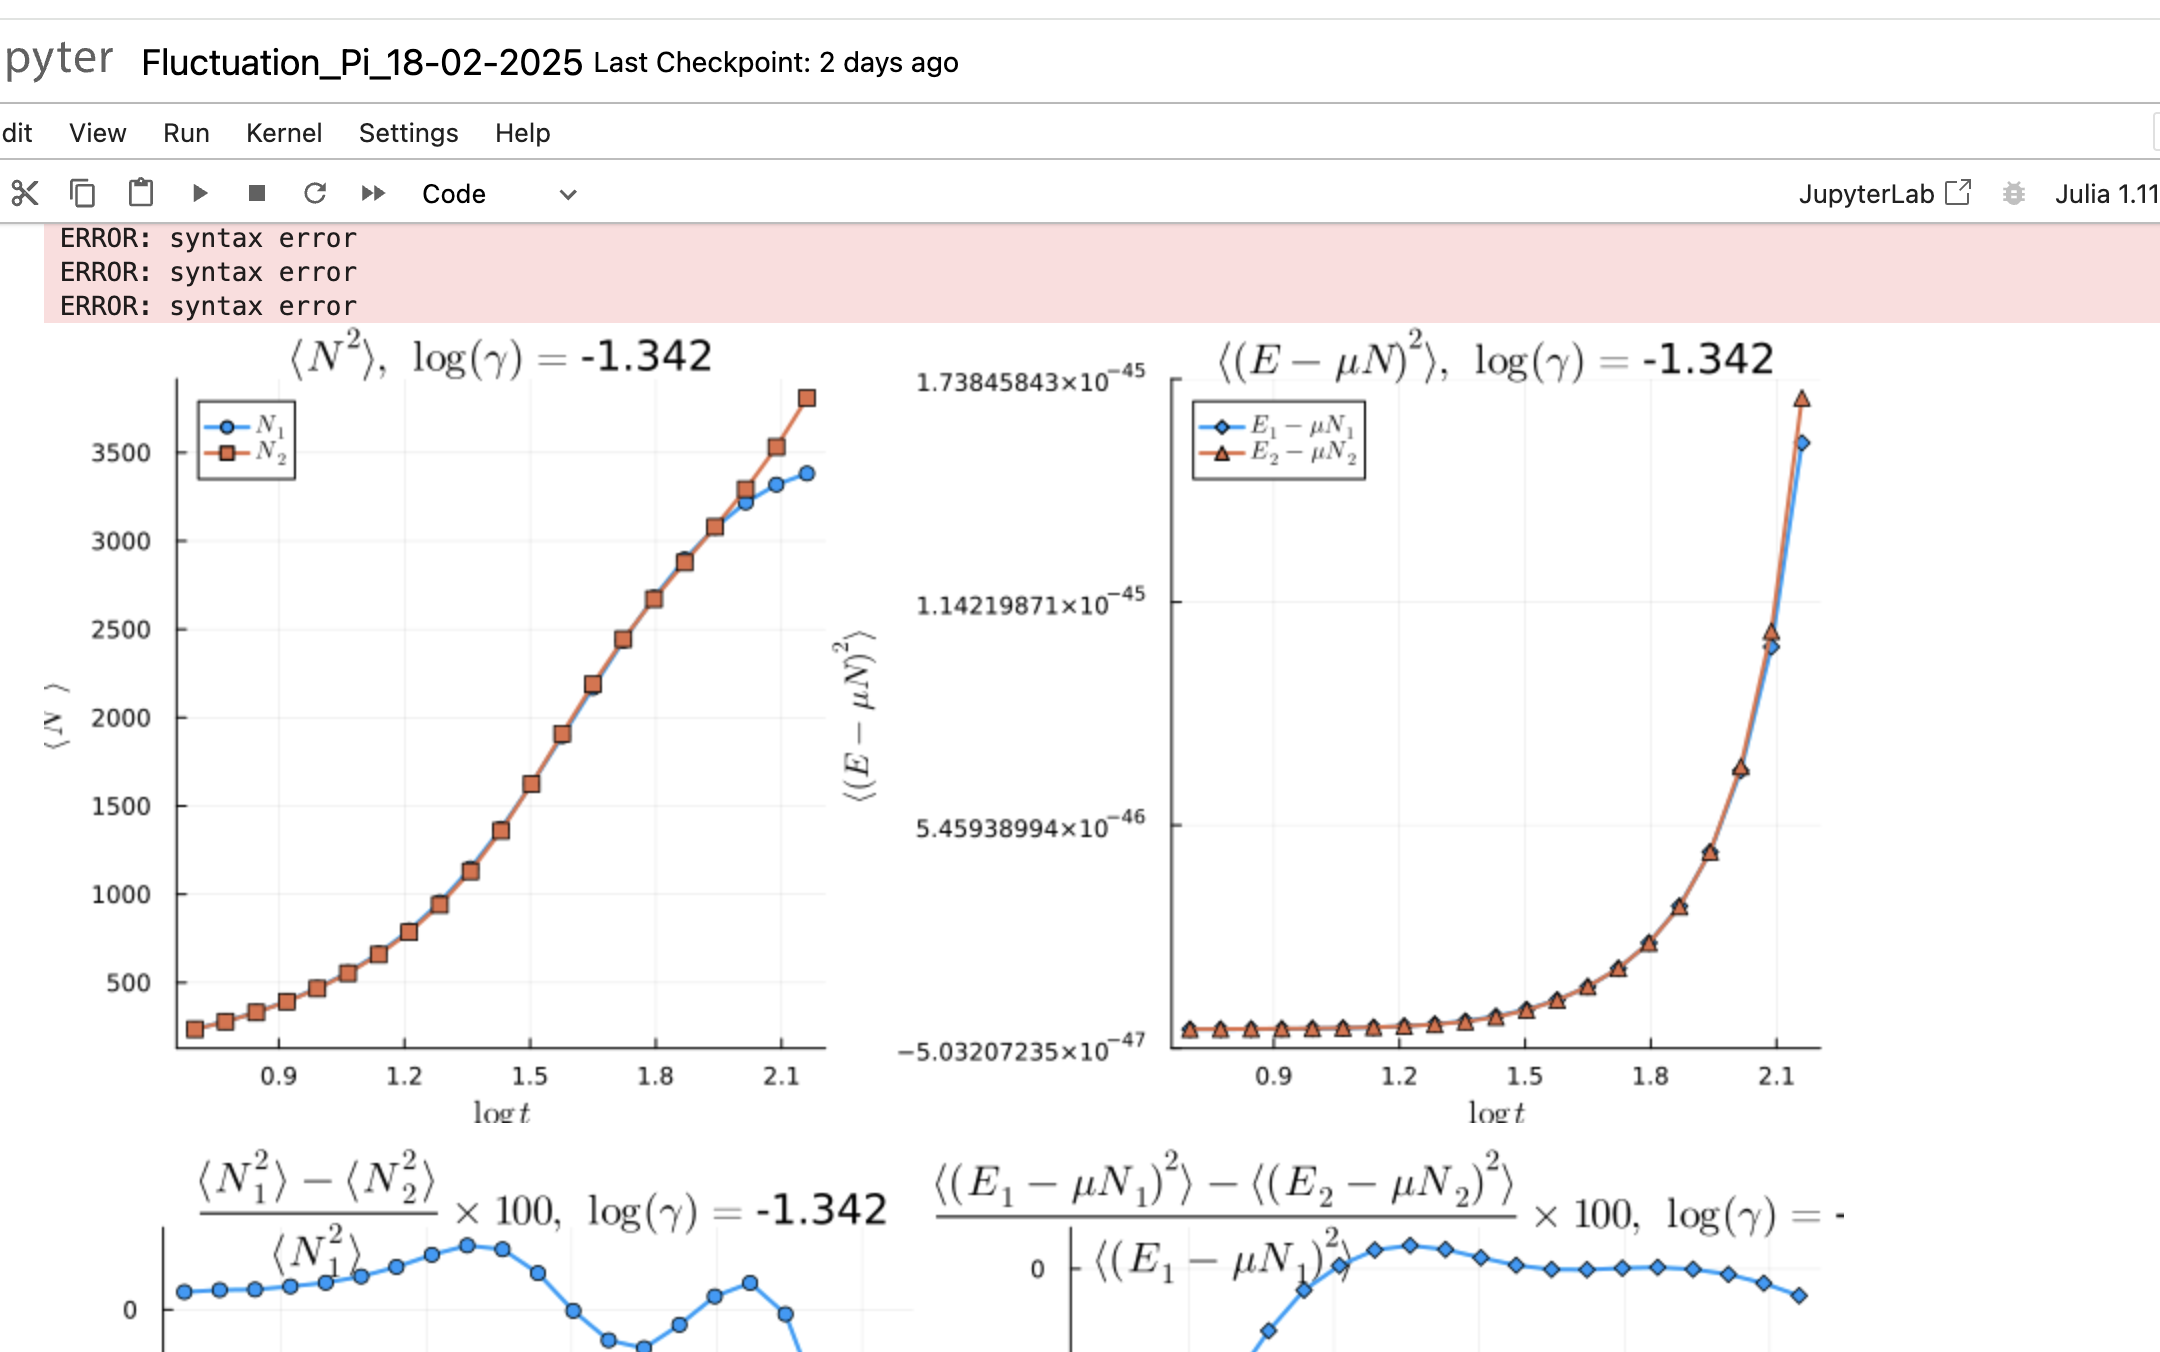
\includegraphics[width=1\textwidth]{Figures/test}

%\begin{aff}
%Donc une a l'ordre un en $\delta \theta (\operator{A}^{(0)})^{-1} %\operator{V}$ 

%\begin{eqnarray*}
%	\langle \delta \Pi ( \theta) \delta \Pi ( \theta') \rangle & = &  ( (\Pi^c_s - \Pi^c)\Pi^c/\Pi^c_s ) ( \theta ) \delta_{\theta, \theta'}/\delta \theta + \mathscr{F}(\theta , \theta' ) ,	
%\end{eqnarray*}

%avec 

%\begin{eqnarray*}
%	\mathscr{F}(\theta , \theta' ) & = & \left [ (\Pi^c_s - \Pi^c )( \theta)  +  (\Pi^c_s - \Pi^c ) ( \theta' )\right ] \frac{\Pi^c}{\Pi^c_s}(\theta)\frac{\Pi^c}{\Pi^c_s}(\theta') \frac{ \Delta( \theta'- \theta )}{ 2 \pi }\\
%	&&  - \left [ (\Pi^c_s - \Pi^c )( \theta)   (\Pi^c_s - \Pi^c ) ( \theta' )\right ] \frac{\Pi^c}{\Pi^c_s}(\theta)\frac{\Pi^c}{\Pi^c_s}(\theta')\int d\theta'' \left (   \frac{ \Pi^c/\Pi^c_s}{\Pi^c_s - \Pi^c} \right )(\theta'') \frac{\Delta(\theta''- \theta)}{2 \pi}\frac{\Delta(\theta''- \theta')}{2 \pi}  	
%\end{eqnarray*}
%\end{aff}



 










